% Created 2019-05-02 Thu 08:44
% Intended LaTeX compiler: pdflatex
\documentclass[10.9pt]{article}
\usepackage[utf8]{inputenc}
\usepackage[T1]{fontenc}
\usepackage{graphicx}
\usepackage{grffile}
\usepackage{longtable}
\usepackage{wrapfig}
\usepackage{rotating}
\usepackage[normalem]{ulem}
\usepackage{amsmath}
\usepackage{textcomp}
\usepackage{amssymb}
\usepackage{capt-of}
\usepackage{hyperref}
\author{Heitor Lourenço Werneck \\{\href{mailto:heitorwerneck@hotmail.com}{heitorwerneck@hotmail.com}}}
\usepackage[portuguese]{babel}
\usepackage{mathtools}
\usepackage[binary-units=true]{siunitx}
\usepackage[top=0.5cm,bottom=1.5cm,left=2cm,right=2cm]{geometry}
\usepackage{mdframed}
\usepackage{listings}
\usepackage[noend]{algpseudocode}
\usepackage{algorithm}
\usepackage{tikz}
\usepackage[font=small,labelfont=bf]{caption} % Required for specifying captions to tables and figures
\usepackage[subrefformat=parens]{subcaption}
\date{\today}
\title{Algoritmos e Estrutura de Dados III (2019-1)\\\medskip
\large Trabalho Prático 2}
\hypersetup{
 pdfauthor={Heitor Lourenço Werneck},
 pdftitle={Algoritmos e Estrutura de Dados III (2019-1)},
 pdfkeywords={},
 pdfsubject={},
 pdfcreator={Emacs 26.1 (Org mode 9.2.2)}, 
 pdflang={Portuguese}}
\begin{document}

\maketitle
\usetikzlibrary{arrows, fit, matrix, positioning, shapes, backgrounds,intersections}


\newcommand{\algruledefaultfactor}{.75}
\newcommand{\algstrut}[1][\algruledefaultfactor]{\vrule width 0pt
depth .25\baselineskip height #1\baselineskip\relax}
\newcommand*{\algrule}[1][\algorithmicindent]{\hspace*{.5em}\vrule\algstrut
\hspace*{\dimexpr#1-.5em}}

\makeatletter
\newcount\ALG@printindent@tempcnta
\def\ALG@printindent{%
    \ifnum \theALG@nested>0% is there anything to print
    \ifx\ALG@text\ALG@x@notext% is this an end group without any text?
    % do nothing
    \else
    \unskip
    % draw a rule for each indent level
    \ALG@printindent@tempcnta=1
    \loop
    \algrule[\csname ALG@ind@\the\ALG@printindent@tempcnta\endcsname]%
    \advance \ALG@printindent@tempcnta 1
    \ifnum \ALG@printindent@tempcnta<\numexpr\theALG@nested+1\relax% can't do <=, so add one to RHS and use < instead
    \repeat
    \fi
    \fi
}%

\patchcmd{\ALG@doentity}{\noindent\hskip\ALG@tlm}{\ALG@printindent}{}{\errmessage{failed to patch}}

\AtBeginEnvironment{algorithmic}{\lineskip0pt}

\newcommand*\Let[2]{\State #1 $\gets$ #2}
\newcommand*\Stateh{\State \algstrut[1]}

\algnewcommand{\IfThenElse}[3]{% \IfThenElse{<if>}{<then>}{<else>}
  \State \algorithmicif\ #1\ \algorithmicthen\ #2\ \algorithmicelse\ #3}
\algnewcommand{\Break}[0]{
  \State \textbf{break}}
\makeatletter
\renewcommand{\ALG@name}{Algoritmo}
\renewcommand{\listalgorithmname}{Lista de\ALG@name s}
\makeatother
\lstset{
  basicstyle=\ttfamily,
  columns=fullflexible,
  frame=single,
  breaklines=true,
  postbreak=\mbox{\textcolor{red}{$\hookrightarrow$}\space},
}
\tikzstyle{block} = [rectangle, draw, 
    text width=5em, text centered]
\tikzstyle{elli} = [draw,ellipse,text width=5em,text centered]
\tikzstyle{decision} = [diamond, draw,text width=4.5em, text badly centered, node distance=3cm, inner sep=0pt]
\tikzstyle{line} = [draw, -latex',dashed]

\newcommand{\myDistance}{2.8cm}
\AtBeginEnvironment{algorithmic}{\footnotesize}
\section{Introdução}
\label{sec:org9ae2663}
Um dos problemas dos pesquisadores de saúde é a análise de imagens oriundas da placenta de bebês, a partir da análise dessas imagens e identificação de certos elementos é possível prevenir uma enorme quantidade de doenças que o bebê poderia ter ao longo de sua vida. O problema pode ser modelado e simplificado como uma matriz \((a_{ij})_{n\times n}\) tal que \(a_{ij} \in \{0(\text{Material líquido}),1(\text{Material sólido})\}\), o objetivo é encontrar a maior submatriz \((s_{ij})_{m\times m}\) com \(m \leq n\) sendo \(s_{ij} = 1\) para \(i=1,...,m \land j=1,...,m\).

A solução é apresentada com força bruta(tentativa e erro), estratégia gulosa, programação dinâmica e \emph{branch and bound}.

A entrada e saída do programa segue o seguinte padrão:
\begin{verbatim}
  Entrada    Saída

             a b c
  1 1 1      a   1 1
  0 1 1  >>  b   1 1 
  0 0 0      c        
\end{verbatim}
\section{Estruturas de Dados}
\label{sec:org3c63b7e}
Deve existir uma variável para guardar o problema, essa variável será definida como:
\begin{verbatim}
int8_t **m;
\end{verbatim}
Foi feito uma estrutura de dados utilizada para auxiliar na solução do problema que descreve o resultado, ou seja uma matriz \((s_{ij})_{m\times m}\) onde \(s_{ij} = 1\) para \(i=1,...,m \land j=1,...,m\).
Sua definição é a seguinte:
\begin{verbatim}
    struct square{
      int order,i,j;
    };
typedef struct square Square;
\end{verbatim}

O padrão de saída de todos paradigmas será essa estrutura.(figura \ref{fig:resultstandard})

\begin{figure}
\centering
\begin{tikzpicture}
\node [draw,rectangle] (brute) {Força bruta};
\node [draw,ellipse,below of=brute] (out1) {Square*};
\node [draw,rectangle,right of=brute,xshift=1.5cm] (greedy) {Guloso};
\node [draw,ellipse,below of=greedy] (out2) {Square*};
\node [draw,rectangle,right of=greedy,xshift=1.5cm] (dynamic) {Dinâmico};
\node [draw,ellipse,below of=dynamic] (out3) {Square*};
\node [draw,rectangle,right of=dynamic,xshift=1.9cm] (bnb) {Branch and Bound};
\node [draw,ellipse,below of=bnb] (out4) {Square*};

% arrows
%\path [->] (brute) -- (out1);
\draw[->] (brute) -- (out1);
\draw[->] (greedy) -- (out2);
\draw[->] (dynamic) -- (out3);
\draw[->] (bnb) -- (out4);
\end{tikzpicture}
\caption{Padronização da saída.}\label{fig:resultstandard}
\end{figure}

Como a estrutura não contem os dados de quais cantos englobam a solução, então é utilizado implicitamente a informação de que a solução engloba a partir do ponto i e j da submatriz quadrada até i+order e j+order. Veja na figura \ref{fig:representacaosquare}.


\begin{figure}
\begin{center}
\begin{tikzpicture}
  \matrix [matrix of math nodes,matrix anchor=west] (m)
          {
            0 &0 &1 \\               
            1 &1 &1 \\               
            0 &1 &1 \\           
          };  
          \scoped[on background layer]
                 {
                   \node[fill=gray!20, fit=(m-2-2)(m-2-3) ]   {};
                   \node[fill=gray!20, fit=(m-3-2)(m-3-3) ]   {};
                 }
                 \draw[color=gray] (m-2-2.north west) -- (m-2-3.north east) -- (m-3-3.south east) -- (m-3-2.south west) -- (m-2-2.north west);

  \matrix [matrix of math nodes,right of=m,xshift=0.3cm,matrix anchor=west] (m2)
          {
            0 &0 &1 \\               
            1 &s_{ij} &s_{i(j+1)} \\               
            0 &s_{(i+1)j} &s_{(i+order)(j+order)} \\           
          };  
          \scoped[on background layer]
                 {
                   \node[fill=gray!20, fit=(m2-2-2)(m2-2-3) ]   {};
                   \node[fill=gray!20, fit=(m2-3-2)(m2-3-3) ]   {};
                 }
                 \draw[color=gray] (m2-2-2.north west) -- (m2-2-3.north east) -- (m2-3-3.south east) -- (m2-3-2.south west) -- (m2-2-2.north west);
%arrow
\draw[implies-implies,double equal sign distance] (m) -- (m2);
\end{tikzpicture}
\end{center}
\caption{Representação dos dados da estrutura Square.}\label{fig:representacaosquare}
\end{figure}

\section{Solução}
\label{sec:org53b621b}
A primeira solução a ser abordada será a de força bruta com tentativa e erro que irá explorar todas possibilidades exaustivamente e garante uma solução ótima.

\subsection{Força bruta (tentativa e erro)}
\label{sec:orgb22d388}

A proposta de força bruta deve explorar todas possibilidades de submatrizes. Como também foi feito com tentativa e erro quando uma tentativa não levar a solução final o passo feito é apagado(encontrar algum 0 em uma submatriz proposta) e vai para próxima tentativa.

Para a verificação se há uma submatriz de ordem m em um dado ponto é necessário o algoritmo \ref{alg:checkSubSquare}.

\begin{algorithm}
\textbf{Input:} matrix :: refToInteger, y, x, area
\caption{Checar existencia de submatriz.}\label{alg:checkSubSquare}
\begin{algorithmic}[1]
\Procedure{checkSubSquare}{}
	\For{$i = y$ to $y+area-1$}
            \For{$j = x$ to $x+area-1$}
		\If{$matrix[i][j] == 0$}
		    \State \Return false
		\EndIf
            \EndFor
	\EndFor
	\State \Return true
  \EndProcedure
\end{algorithmic}
\end{algorithm}

Porém quando se está expandindo a partir de um ponto só é preciso verificar os cantos logo um outro algoritmo pode ser criado somente para a verificação de 1's no canto para evitar redundância de verificação.(algoritmo \ref{alg:checkSubSquareCorner})

\begin{algorithm}
\textbf{Input:} matrix :: refToInteger, y, x, area, corner
\caption{Checar existencia de submatriz.}\label{alg:checkSubSquareCorner}
\begin{algorithmic}[1]
\State \textbf{enum} Moves\{LeftBottom=0,LeftTop,RightTop,RightBottom\}
\Procedure{checkSubSquareCorner}{} \Comment{O(area)}
\IfThenElse{$corner==LeftBottom \lor corner==RightBottom$}{$yAdd=area-1$}{$yAdd=0$}
\IfThenElse{$corner==RightTop \lor corner==RightBottom$}{$xAdd=area-1$}{$xAdd=0$}
	\For{$i = x$ to $x+area$}
	    \If{$matrix[y+yAdd][i] == 0$}
		\State \Return false
	    \EndIf
	\EndFor
	\For{$i = y$ to $y+area$}
	    \If{$matrix[i][x+xAdd] == 0$}
		\State \Return false
	    \EndIf
	\EndFor
	\State \Return true
  \EndProcedure
\end{algorithmic}
\end{algorithm}

Então o algoritmo que testa todas possibilidades com auxilio do algoritmo \ref{alg:checkSubSquareCorner} será o algoritmo \ref{alg:maxSubSquareBruteForce}.

\begin{algorithm}
\textbf{Input:} matrix :: refToInteger, n
\caption{Acha a maior submatriz com força bruta.}\label{alg:maxSubSquareBruteForce}
\begin{algorithmic}[1]
\Procedure{maxSubSquareBruteForce}{}
    \State maxSqr = \{0,0,0\}
            \For{$i = 0$ to $n-1$}\label{alg:maxSubSquareBruteForce:for1}
		\For{$j = 0$ to $n-1$}\label{alg:maxSubSquareBruteForce:for2}
		\For{$area = 1$ to $n$}\label{alg:maxSubSquareBruteForce:for3}
		\If{$i <= n-area \land j <= n-area \land checkSubSquareCorner(m,i, j,area,RightBottom)$}\label{alg:maxSubSquareBruteForce:up2}
		    \If{$maxSqr.order < area$}
			\State maxSqr.order = area
			\State maxSqr.i = i
			\State maxSqr.j = j
			\EndIf
			\Else
			\Break
		    \EndIf
                \EndFor
		\EndFor
            \EndFor
	\State \Return maxSqr
  \EndProcedure
\end{algorithmic}
\end{algorithm}

O algoritmo \ref{alg:maxSubSquareBruteForce} começa zerando os campos da matriz resultado, depois dois laços aninhados percorrem a matriz nos índices i e j. Na linha \ref{alg:maxSubSquareBruteForce:for3} é passado por todas ordens possíveis da matriz até que alguma propriedade não seja valida que é checado na linha \ref{alg:maxSubSquareBruteForce:up2}(no código em c há otimizações), se o tamanho da submatriz a ser testada violar o tamanho da matriz ou se os cantos da matriz não estiverem preenchidos por 1 então começa a testar a próxima célula caso exista e durante esse processo se a ordem obtida for maior que a atual então guarda essa submatriz.

\subsection{Branch and bound}
\label{sec:org8305cfe}
O algoritmo força bruta por tentativa e erro pode ainda ser melhorado utilizando branch and bound \cite{Lawler1966}. O objetivo do algoritmo é eliminar verificações de áreas que não serão obtidas uma ordem maior de submatriz que a atual, desse modo cortando grande parte do problema. Isso pode ser feito facilmente somente trocando o ponto de parada do primeiro laço (linha \ref{alg:maxSubSquareBruteForce:for1}) de \(n-1\) para \(n-maxSqr.order-1\) e a mesma coisa para o segundo laço (linha \ref{alg:maxSubSquareBruteForce:for2}).
\subsection{Estratégia gulosa}
\label{sec:org556f2f5}
Para esse problema é possível dar diversas estratégias gulosas a partir do critério global de otimalidade que é: a sub matriz quadrada de 1 deve ser a maior possível. \cite{curtis03_class_greed_algor}

Para maximizar a obtenção de uma solução ótima é importante ater-se a boas estratégias gulosas.

Na busca por uma estratégia gulosa é interessante explorar as propriedades de uma solução ótima, a solução ótima possui uma alta densidade de 1's em um só local.

Um critério de otimalidade local: o ponto escolhido para se expandir deve ter a linha com maior quantidade de 1's em sequência(um ponto que possivelmente está dentro uma submatriz ótima). E esse mesmo pensamento pode ser derivado para colunas e diagonais paralelas a diagonal principal e secundária. 

E adicionando todos esses critérios e formulando uma estratégia que engloba os 4 poderia ser feito um algoritmo que cria 4 matrizes, que nelas estão somados 1's em sequência em suas respectivas direções e apos a criação soma as 4 e acha a maior célula, essa célula seria uma célula com alta concentração de 1's que pode-se dizer que é bastante robusto, porém a complexidade de espaço deixaria o algoritmo pouco interessante por conta de sua performance visto que o algoritmo de programação dinâmica teria a mesma complexidade de espaço como será possível observar mais a frente.

Logo a estratégia a ser utilizada para achar um ponto que possivelmente está dentro de uma submatriz ótima irá se ater a propriedade simples de linha com maior quantidade de 1's em sequência e coluna com maior quantidade de 1's em sequência. Com a linha e a coluna obtida basta fazer um cruzamento de linha e coluna para achar o ponto para se expandir.

É importante notar que para uma matriz da forma
\begin{table}[htbp]
\centering
\begin{tabular}{rrrrr}
0 & 1 & 0 & 1 & 1\\
0 & 1 & 0 & 1 & 1\\
1 & 1 & 1 & 1 & 1\\
0 & 1 & 0 & 0 & 0\\
0 & 1 & 0 & 0 & 0\\
\end{tabular}
\quad
\begin{tabular}{rrrrr}
0 & 1 & 1 & 1 & 1\\
1 & 0 & 0 & 0 & 0\\
1 & 0 & 1 & 1 & 1\\
1 & 0 & 1 & 1 & 1\\
1 & 0 & 1 & 1 & 1\\
\end{tabular}
\caption{Casos de solução ruim pela estratégia gulosa.}
\end{table}

a estratégia gulosa não irá apresentar uma solução ótima.

O algoritmo \(maxSubSquareGreedy\) (\ref{alg:maxSubSquareGreedy}) é dependente da função \(maxSubSquarePoint\), ou seja, é necessário outro processo além do de escolha do ponto, é necessário expandir por esse ponto para obter a maior matriz nesse ponto (etapa de construção da solução).

\begin{algorithm}
\textbf{Input:} matrix :: refToInteger, n
\caption{Acha a maior submatriz com uma estratégia gulosa.}\label{alg:maxSubSquareGreedy}
\begin{algorithmic}[1]
\Procedure{maxSubSquareGreedy}{}
\State i,j,bestLine=0,bestColumn=0,bestLineQnt=0,bestColumnQnt=0,tempQnt=0

\For{$i=0$ to $n$}
    \State $tempQnt=0$
    \For{$j=0$ to $n$}
        \State $tempQnt+= matrix[i][j]$
        \If{$matrix[i][j] == 0$}
            \If{$tempQnt>bestLineQnt$}
                \State $bestLineQnt = tempQnt$
                \State $bestLine = i$
            \EndIf
            \State $tempQnt=0$
        \EndIf
    \EndFor
    \If{$tempQnt>bestLineQnt$}
	\State $bestLineQnt = tempQnt$
	\State $bestLine = i$
    \EndIf
    \State $tempQnt=0$
    \For{$j=0$ to $n$}
        \State $tempQnt+= matrix[i][j]$
        \If{$matrix[i][j] == 0$}
            \If{$tempQnt>bestColumnQnt$}
                \State $bestLineQnt = tempQnt$
                \State $bestLine = i$
            \EndIf
            \State $tempQnt=0$
        \EndIf
    \EndFor
    \If{$tempQnt>bestLineQnt$}
	\State $bestLineQnt = tempQnt$
	\State $bestLine = i$
    \EndIf
\EndFor

\State $maxSqr.order=m[bestLine][bestColumn]$
\State $maxSqr.i = bestLine$
\State $maxSqr.j = bestColumn$

\If{$m[bestLine][bestColumn]$}
\State $subSquarePoint(m,n,maxSqr)$
\EndIf
\State \Return $maxSqr$
\EndProcedure
\end{algorithmic}
\end{algorithm}

Para expandir por um ponto é necessário definir os sentidos de tentativa de crescimento. Por exemplo: cresce o máximo possível no canto inferior esquerdo depois esquerdo superior, direito superior e direito inferior. Esse processo é ilustrado na figura \ref{fig:greedyprocess} (matriz quadrada de ordem 3).

Na matriz da figura \ref{fig:greedyprocess} o primeiro movimento falha, o segundo também e no terceiro já é possível expandir a matriz(movimento para a direita superior) e incrementado no conjunto solução, o segundo movimento para essa mesma direção já não é possível pois acessa posições invalidas logo tenta o outro movimento que também é invalido e então termina e retorna o conjunto solução que é uma matriz 2x2. Veja o algoritmo \ref{alg:subSquarePoint}.

\begin{figure}
\begin{center}
\begin{tikzpicture}[node distance = 2cm, auto]

  \matrix [matrix of math nodes,left delimiter={[},right delimiter={]},matrix anchor=west] (m1)
          {
            0 &1 &1 \\               
            1 &1 &1 \\               
            0 &0 &0 \\           
          };  
          \scoped[on background layer]
                 {
                   \node[fill=gray!20, fit=(m1-1-2)(m1-3-2) ]   {};
                   \node[fill=gray!20, fit=(m1-2-1)(m1-2-3) ]   {};
                 }
		 
  \matrix [right of = m1,matrix of math nodes,left delimiter={[},right delimiter={]},matrix anchor=west] (mini1)
          {
	    x & x & x& x \\
            0 &1 &1 & x \\               
            1 &1 &1 & x \\               
            0 &0 &0 & x \\           
          };  

	  \draw[dashed,color=red] (mini1-3-1.north west) -- (mini1-3-2.north east) -- (mini1-4-2.south east) -- (mini1-4-1.south west) -- (mini1-3-1.north west);


  \matrix [right of = mini1,matrix of math nodes,left delimiter={[},right delimiter={]},matrix anchor=west] (m2)
          {
	    x & x & x& x \\
            0 &1 &1 & x \\               
            1 &1 &1 & x \\               
            0 &0 &0 & x \\           
          };  
                 \draw[dashed,color=red] (m2-2-1.north west) -- (m2-2-2.north east) -- (m2-3-2.south east) -- (m2-3-1.south west) -- (m2-2-1.north west);
                 \draw[dashed,color=red] (m2-3-1.north west) -- (m2-3-2.north east) -- (m2-4-2.south east) -- (m2-4-1.south west) -- (m2-3-1.north west);

  \matrix [right of = m2,matrix of math nodes,left delimiter={[},right delimiter={]},matrix anchor=west] (m3)
          {
	    x & x & x& x \\
            0 &1 &1 & x \\               
            1 &1 &1 & x \\               
            0 &0 &0 & x \\           
          };  
          \scoped[on background layer]
                 {
                   \node[fill=green!20, fit=(m3-2-2)(m3-2-3) ]   {};
                   \node[fill=green!20, fit=(m3-3-2)(m3-3-3) ]   {};
                 }
                 \draw[dashed,color=red] (m3-2-1.north west) -- (m3-2-2.north east) -- (m3-3-2.south east) -- (m3-3-1.south west) -- (m3-2-1.north west);
                 \draw[dashed,color=red] (m3-3-1.north west) -- (m3-3-2.north east) -- (m3-4-2.south east) -- (m3-4-1.south west) -- (m3-3-1.north west);
                 \draw[color=green] (m3-2-2.north west) -- (m3-2-3.north east) -- (m3-3-3.south east) -- (m3-3-2.south west) -- (m3-2-2.north west);


  \matrix [right of = m3,matrix of math nodes,left delimiter={[},right delimiter={]},matrix anchor=west] (m4)
          {
	    x & x & x& x \\
            0 &1 &1 & x \\               
            1 &1 &1 & x \\               
            0 &0 &0 & x \\           
          };  
          \scoped[on background layer]
                 {
                   \node[fill=green!20, fit=(m4-2-2)(m4-2-3) ]   {};
                   \node[fill=green!20, fit=(m4-3-2)(m4-3-3) ]   {};
                 }
                 \draw[dashed,color=red] (m4-2-1.north west) -- (m4-2-2.north east) -- (m4-3-2.south east) -- (m4-3-1.south west) -- (m4-2-1.north west);
                 \draw[dashed,color=red] (m4-3-1.north west) -- (m4-3-2.north east) -- (m4-4-2.south east) -- (m4-4-1.south west) -- (m4-3-1.north west);
                 \draw[color=green] (m4-2-2.north west) -- (m4-2-3.north east) -- (m4-3-3.south east) -- (m4-3-2.south west) -- (m4-2-2.north west);
                 \draw[dashed,color=red] (m4-1-2.north west) -- (m4-1-4.north east) -- (m4-3-4.south east) -- (m4-3-2.south west) -- (m4-1-2.north west);


  \matrix [right of = m4,matrix of math nodes,left delimiter={[},right delimiter={]},matrix anchor=west] (m5)
          {
	    x & x & x& x \\
            0 &1 &1 & x \\               
            1 &1 &1 & x \\               
            0 &0 &0 & x \\           
          };  
          \scoped[on background layer]
                 {
                   \node[fill=green!20, fit=(m5-2-2)(m5-2-3) ]   {};
                   \node[fill=green!20, fit=(m5-3-2)(m5-3-3) ]   {};
                 }
                 \draw[dashed,color=red] (m5-2-1.north west) -- (m5-2-2.north east) -- (m5-3-2.south east) -- (m5-3-1.south west) -- (m5-2-1.north west);
                 \draw[dashed,color=red] (m5-3-1.north west) -- (m5-3-2.north east) -- (m5-4-2.south east) -- (m5-4-1.south west) -- (m5-3-1.north west);
                 \draw[color=green] (m5-2-2.north west) -- (m5-2-3.north east) -- (m5-3-3.south east) -- (m5-3-2.south west) -- (m5-2-2.north west);
                 \draw[dashed,color=red] (m5-1-2.north west) -- (m5-1-4.north east) -- (m5-3-4.south east) -- (m5-3-2.south west) -- (m5-1-2.north west);
                 \draw[dashed,color=red] (m5-2-2.north west) -- (m5-2-4.north east) -- (m5-4-4.south east) -- (m5-4-2.south west) -- (m5-2-2.north west);


		 \node[above of = m3,yshift=-0.7cm] (comment2) {Processo de construção};
\node[above of = m1,yshift=-0.7cm] {Linha e coluna escolhidas};
\end{tikzpicture}
\end{center}
\caption{Processo guloso.}\label{fig:greedyprocess}
\end{figure}

\begin{algorithm}
\textbf{Input:} matrix :: refToInteger, n,maxSqr
\caption{Expande a partir de um ponto.}\label{alg:subSquarePoint}
\begin{algorithmic}[1]
\Procedure{subSquarePoint}{}
\State $bestLine=maxSqr.i,bestColumn=maxSqr.j,right=bestColumn,left=bestColumn,top=bestLine,bottom=bestLine,moved$
\State $corner =$ LeftBottom
\While{$corner <=$ RightBottom}
\State Faz um movimento
\If{Se foi um movimento valido}
    \If{checkSubSquare(matriz,top,left,right-left+1,corner)}
        \State Adiciona o pedaço valido descoberto ao conjunto solução
    \Else
       \State Desfaz movimento
    \EndIf
\Else
    \State Proximo sentido de movimento
\EndIf
\EndWhile
\EndProcedure
\end{algorithmic}
\end{algorithm}

Seria possível obter a maior matriz que engloba um ponto dado fazendo todas combinações de ordem movimentos porém necessitaria de uma avaliação de qual a solução maior e isso pode ser avaliado como um processo não guloso, logo no algoritmo é utilizado uma ordem arbitrária.

Outra proposta para se achar boas soluções seria a execução de todas combinações de estratégias gulosas e checar qual a estratégia da a maior submatriz, desse modo poderia-se chegar a soluções possivelmente melhores. A figura \ref{fig:combgulosa} ilustra esse processo.

\begin{figure}[htbp]
\centering
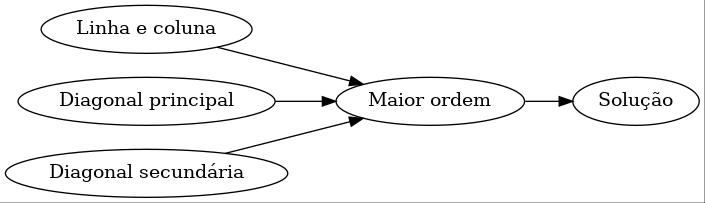
\includegraphics[width=0.44\textwidth]{combgulosa.jpg}
\caption{Combinação de estratégias gulosas.\label{fig:combgulosa}}
\end{figure}

\subsection{Programação dinâmica}
\label{sec:orgafe0f9a}
O paradigma de programação para ser aplicado nesse problema, mais rápido e eficiente que o força bruta e que, ao contrário da estratégia gulosa apresentada, sempre alcança solução ótima é o paradigma de programação dinâmica.

Visto que esse problema apresenta sobreposição dos subproblemas o algoritmo de força bruta trabalha mais que o necessário. O algoritmo de programação dinâmica a ser apresentado não irá apresentar esse problema.

Resolvendo o problema recursivamente \cite{laaksonen17_introd} e guardando os valores das submatrizes em uma tabela é exibido a propriedade de subestrutura ótima \cite{cormen09_introd} desse problema.

\begin{tabular}{ | l | c | r |}
  \hline
  1 & 1 & 1 \\ \hline
  1 & 1 & 1 \\ \hline
  1 & 1 & 1 \\ 
  \hline
\end{tabular}
$\implies$
\quad
\begin{tabular}{ | l | c | r |}
  \hline
   &  &  \\ \hline
   &  &  \\ \hline
   &  &  \\ 
  \hline
\end{tabular}
\quad
\begin{tabular}{ | l | c | r |}
  \hline
  1 & 1 & 1 \\ \hline
  1 & 2 &  \\ \hline
  1 &  &  \\ 
  \hline
\end{tabular}
\quad
\begin{tabular}{ | l | c | r |}
  \hline
  1 & 1 & 1 \\ \hline
  1 & 2 & 2 \\ \hline
  1 &  &  \\ 
  \hline
\end{tabular}
\quad
\begin{tabular}{ | l | c | r |}
  \hline
  1 & 1 & 1 \\ \hline
  1 & 2 & 2 \\ \hline
  1 & 2 &  \\ 
  \hline
\end{tabular}
\quad
\begin{tabular}{ | l | c | r |}
  \hline
  1 & 1 & 1 \\ \hline
  1 & 2 & 2 \\ \hline
  1 & 2 & 3 \\ 
  \hline
\end{tabular}

É possível notar que os problemas maiores dependem dos problemas menores para serem resolvidos. 
Então o segundo passo é descrever o valor de uma solução ótima:

\begin{equation}\label{eq:casodinamico}
m[i,j] = 
\begin{cases}
0 & \text{if $m[i,j] = 0 \land (i = 0 \lor j = 0) $ }\\
1 & \text{if $m[i,j] = 1 \land (i = 0 \lor j = 0) $ }\\
0 & \text{if $m[i,j] = 0 \land i \neq 0 \land j \neq 0 $ }\\
1+min(m[i-1,j],m[i-1,j-1],m[i,j-1]) & \text{if $m[i,j] = 1 \land i \neq 0 \land j \neq 0$}\\
\end{cases}
\end{equation}
\begin{equation}
\begin{aligned}
m = max(m[i,j])\\
resolver(A_{n\times n})=(s_{ij})_{m\times m}\\
\end{aligned}
\end{equation}

Essa é toda a base necessária para escrever o algoritmo que resolve o problema.

O algoritmo com programação dinâmica (\ref{alg:maxSubSquareDynamic}) começara criando um auxiliar que guardará a maior submatriz encontrada até o momento e uma tabela de ordem \(n\times n\) para guardar as soluções, após isso é necessário primeiro completar a tabela na sua primeira coluna e linha, pois são problemas elementares, para então começar a análise dos problemas que sobrepõem os outros problemas.

O próximo passo do algoritmo é completar a tabela passando em cada linha por todas suas colunas começando por uma linha a baixo e uma coluna a frente em todas linhas, e basta utilizar a lógica dos dois últimos casos da equação \eqref{eq:casodinamico} para aplicar valores em cada célula \((i,j)\). Para guardar a maior ordem de uma submatriz basta verificar se um valor de uma solução é maior que a submatriz encontrada até então ou não (linha \ref{alg:maxSubSquareDynamic:maxorder}), se for guarda a sua ordem e índice, visto que a solução nesse algoritmo é construída de cima para baixo na tabela então o índice é respectivo ao canto inferior direito, mas nesse trabalho esta sendo usado o padrão de que o índice se refere ao canto superior esquerdo logo é feito uma normalização nas linhas \ref{alg:maxSubSquareDynamic:norm1} e \ref{alg:maxSubSquareDynamic:norm2}.

\begin{algorithm}
\textbf{Input:} matrix :: refToInteger, n
\caption{Acha a maior submatriz com programação dinâmica.}\label{alg:maxSubSquareDynamic}
\begin{algorithmic}[1]
\Procedure{maxSubSquareDynamic}{}
\State $maxSqr.order=0; maxSqr.i=0;maxSqr.j=0$
\State $table[n][n]$\label{alg:maxSubSquareDynamic:table}
\For{$i=0$ to $n$}
\State $table[i][0] = matrix[i][0]$
\State $table[0][i] = matrix[0][i]$
\If{$table[i][0] == 1$}
    \State $maxSqr.order=1$
    \State $maxSqr.i=i$
    \State $maxSqr.j=0$
\EndIf
\If{$table[i][0] == 1$}
    \State $maxSqr.order=1$
    \State $maxSqr.i=0$
    \State $maxSqr.j=i$
\EndIf
\EndFor

	\For{$i = 1$ to $n$}
            \For{$j = 1$ to $n$}
		\If{$matrix[i][j] == 0$}
		    \State $table[i][j] = 0$
		\Else
		    \State $table[i][j] = 1+min(table[i-1][j],table[i-1][j-1],table[i][j-1])$
		    \If{$table[i][j] > maxSqr.order$}\label{alg:maxSubSquareDynamic:maxorder}
		    \State $maxSqr.order=table[i][j]$
		    \State $maxSqr.i=i-maxSqr.order+1$\label{alg:maxSubSquareDynamic:norm1}
		    \State $maxSqr.j=j-maxSqr.order+1$\label{alg:maxSubSquareDynamic:norm2}
		    \EndIf
		\EndIf
            \EndFor
	\EndFor
	\State \Return maxSqr
  \EndProcedure
\end{algorithmic}
\end{algorithm}

\subsection{Programa principal}
\label{sec:orgae5522d}
O programa principal é feito em função dos algoritmos obtidos que resolvem o problema de diferentes formas. A figura \ref{fig:programaprincipal} ilustra o programa principal.
\begin{figure}
\centering
\begin{tikzpicture}[node distance = \myDistance, auto]
\node [block] (exe) {Execução};
\node [block,right of = brute] (args) {Leitura dos argumentos e abertura dos arquivos};
\node [draw,ellipse,above of = args,xshift=-2cm,yshift = -\myDistance+2cm] (paradigma) {$paradigma \in \{b,d,g,n\}$};
\node [draw,ellipse,right of = args,yshift=2cm] (erro1) {Erro};
\node [block,right of = args] (mfile) {Aloca em uma variável a matriz do arquivo};
\node [draw,ellipse,above right of = mfile,xshift=0.3cm] (varm) {$m[n][n]$};
\node [block,right of = mfile,xshift=2cm,yshift=2cm] (brute) {Força bruta};
\node [block,below of = brute,yshift = \myDistance-1cm] (greedy) {Guloso};
\node [block,below of = greedy,yshift = \myDistance-1cm] (dynamic) {Dinâmico};
\node [block,below of = dynamic,yshift = \myDistance-1cm] (bnb) {Branch and Bound};
\node [block,right of = dynamic] (solucao) {Imprime solução obtida};
\node [block,right of = solucao] (desaloca) {Desaloca variáveis};
% arrows
\path [line] (exe) -- (args);
\path [line] (args) -- (erro1) node [midway, yshift= -0.1cm ,above] (TextNode) {Falha};
\path [line] (args) -- (mfile) node [midway, yshift= -0.1cm ,above] (TextNode) {Sucesso};
\path [line] (args) -- (paradigma);
\path [line] (mfile) -- (varm);
\path [line] (mfile) -- (brute) node [midway, yshift= -0.1cm ,above] (TextNode) {paradigma = b};
\path [line] (mfile) -- (greedy) node [midway, yshift= -0.1cm ,above] (TextNode) {paradigma = g};
\path [line] (mfile) -- (dynamic) node [midway, yshift= -0.1cm ,above] (TextNode) {paradigma = d};
\path [line] (mfile) -- (bnb) node [midway, yshift= -0.1cm ,above] (TextNode) {paradigma = n};
\path [line] (brute) -- (solucao);
\path [line] (greedy) -- (solucao);
\path [line] (dynamic) -- (solucao);
\path [line] (bnb) -- (solucao);
\path [line] (solucao) -- (desaloca);
\end{tikzpicture}
\caption{Programa principal.}\label{fig:programaprincipal}
\end{figure}
\section{Análise de complexidade}
\label{sec:org6d79465}
\subsection{Complexidade de tempo}
\label{sec:org4ac4d9d}
Antes da análise de complexidade é importante definir a variável que irá dar a complexidade do algoritmo.
\begin{equation}
\underbrace{n}_{\parbox{3.65cm}{quantidade de colunas ou linhas da matriz}} \in \mathbb{N}\\
\end{equation}
\subsubsection{Força bruta}
\label{sec:org638b97c}
Como o algoritmo \ref{alg:maxSubSquareBruteForce} depende do algoritmo de checar os cantos (algoritmo \ref{alg:checkSubSquareCorner}), então é necessário sua análise inicialmente.


\begin{equation}
\begin{aligned}\label{eq:checkSubSquareCorner}
checkSubSquareCorner(area)\in \sum_{i=1}^{area} O(1) + \sum_{i=1}^{area} O(1)=area\cdot O(1)+area\cdot O(1)=area\cdot O(1)\\
\therefore checkSubSquareCorner(area) \in O(area)
\end{aligned}
\end{equation}

\begin{equation}
\begin{aligned}
makSubSquareBruteForce(n)\in \sum_{i=1}^{n}\sum_{j=1}^{n}\sum_{area=1}^{n} O(area)=O(\sum_{i=1}^{n}\sum_{j=1}^{n}\sum_{area=1}^{n} area) \\
O(\sum_{i=1}^{n}\sum_{j=1}^{n} \frac{n\cdot (n+1)}{2}) = O(\frac{n^3\cdot (n+1)}{2}) \\
\therefore maxSubSquareBruteForce(n) \in O(n^4)
\end{aligned}
\end{equation}
\subsubsection{Branch and bound}
\label{sec:org24f68a9}
A abordagem em \emph{branch and bound} é complexa, para fazer sua análise detalhada é difícil pois os limites do laço podem mudar ou não a cada iteração. Mas de qualquer maneira foi provado que sua complexidade é \(O(n^4)\) porém na pratica seu desempenho deve ser muito melhor.
\begin{equation}
  \begin{aligned}
    maxSubSquareBranchnBound(n)\\
    \sum_{i=1}^{n-Sqr.order}\sum_{j=1}^{n-Sqr.order}\sum_{area=1}^{n} O(area)=O(\sum_{i=1}^{n-Sqr.order}\sum_{j=1}^{n-Sqr.order}\sum_{area=1}^{n} area) \\
    O(\sum_{i=1}^{n-Sqr.order}\sum_{j=1}^{n-Sqr.order} \frac{n\cdot (n+1)}{2}); Sqr.order \in \{x : x \in \mathbb{N^{*}} \land  x \leq n\}\\
    n-Sqr.order; \exists (c \in \mathbb{N^{*}}) \exists (m \in \mathbb{N^{*}}) \forall (n \geq m) : 0 \leq n-Sqr.order \leq c\cdot n\\
    m = 1; c = 1 \implies 0 \leq n-Sqr.order \leq n \implies n-Sqr.order \in O(n)\\
    O(\frac{(n-Sqr.order)^2\cdot n\cdot (n+1)}{2}) \in  O(\frac{n^3\cdot (n+1)}{2}) \therefore maxSubSquareBranchnBound(n) \in O(n^4)
  \end{aligned}
\end{equation}

\subsubsection{Algoritmo guloso}
\label{sec:org22f8e4a}
O pior caso do algoritmo \(subSquarePoint\) (\ref{alg:subSquarePoint}) ocorrerá quando ele continua adicionando pedaços validos e no máximo pode existir \(O(n^2)\) pedaços, então o algoritmo \(maxSubSquareGreedy\) é \(O(n^2)\) como é mostrado.
\begin{equation}
  \begin{aligned}\label{eq:subSquarePoint}
    \therefore subSquarePoint(n) \in O(n^2)
  \end{aligned}
\end{equation}
\begin{equation}
  \begin{aligned}\label{eq:maxSubSquareGreedy}
  maxSubSquareGreedy(n)\in O(max(\sum_{i=0}^{n}\sum_{j=0}^{n} 1,n^2))\\
    \therefore maxSubSquareGreedy(n) \in O(n^2)
  \end{aligned}
\end{equation}
\subsubsection{Programação dinâmica}
\label{sec:orgde93901}

\begin{equation}
  \begin{aligned}
    maxSubSquareDynamic(n) \in \sum_{i=0}^{n} O(1)+\sum_{i=0}^{n}\sum_{j=0}^{n} O(1) = O(max(\sum_{i=0}^{n} 1,\sum_{i=1}^{n}\sum_{j=1}^{n} 1)) = O(n^2)\\
    \therefore maxSubSquareDynamic(n) \in O(n^2)
  \end{aligned}
\end{equation}
\subsubsection{Programa principal}
\label{sec:orga46512a}
A análise do programa principal será feita com base na figura \ref{fig:programaprincipal}. É intuitivo pensar que o passo de alocar em uma variável a matriz que foi entrada no arquivo tem complexidade \(O(n^2)\), apos isso um dos algoritmos será executado, considerando o pior caso então será \(O(max(n^2,n^4)) \implies O(n^4)\), logo a complexidade do programa principal será \(O(n^4)\).
\subsection{Complexidade de espaço}
\label{sec:orgfe83b38}
Antes de se fazer a análise de complexidade de espaço é preciso evidenciar que os algoritmos que possuem em sua lista de parâmetros uma referência para um vetor não apresentará complexidade de espaço relacionada com o espaço ocupado por esse valor referenciado(Ex. \(O(n^c), c \in \mathbb{N}\)) pois o parâmetro guarda uma constante(referência para o vetor) ou seja a complexidade de espaço é constante.\cite{spacecomplexitypointer}
\subsubsection{Força bruta}
\label{sec:org7bcdd3b}
 O algoritmo força bruta utiliza a função \textbf{checkSubSquareCorner} logo é necessário analisar sua complexidade de espaço, essa função não cria um vetor ou algo parecido, somente usa um espaço constante de espaço logo sua complexidade é O(1).
O algoritmo força bruta apresenta complexidade de espaço \(O(1)\) da mesma forma pois utiliza uma quantidade de espaço constante, e como já comentado só há uma referência a uma matriz \(n\times n\) e essa referência é \(O(1)\).
\subsubsection{Branch and bound}
\label{sec:orgb477a6b}
A abordagem em \emph{branch and bound} é bem similar ao força bruta, é fácil identificar que esse algoritmo também tem complexidade de espaço \(O(1)\).

\subsubsection{Algoritmo guloso}
\label{sec:org29b7bb9}
A função \textbf{subSquarePoint} utiliza a função \textbf{checkSubSquareCorner} que tem complexidade de espaço \(O(1)\) e não há nenhum crescimento de espaço na função \textbf{subSquarePoint} logo sua complexidade também é \(O(1)\).
Como a função \textbf{subSquarePoint} é \(O(1)\) então a complexidade de espaço da função \textbf{maxSubSquareGreedy} é \(O(1)\) também pois não há nenhuma variavel com tamanho dependente da entrada.
\subsubsection{Programação dinâmica}
\label{sec:org123977e}
O algoritmo dinâmico apresenta complexidade de espaço \(O(n^2)\) pois na linha \ref{alg:maxSubSquareDynamic:table} há a criação de uma tabela auxiliar com tamanho dependente da entrada de ordem \(n^2\).
\subsubsection{Programa principal}
\label{sec:org98651e4}
Com base na figura \ref{fig:programaprincipal} o passo de alocar uma variável que tem tamanho \(n^2\) implicará em uma complexidade de espaço de \(O(n^2)\), junto com o resto do programa \(O(max(n^2,1,1,n^2,1)) = O(n^2)\). Logo a complexidade de espaço do programa principal é \(O(n^2)\).


\subsection{Análise Geral}
\label{sec:orgf080b3f}
A tabela \ref{tab:org6b408f4} mostra todas complexidades obtidas, com ela pode-se ver que o melhor algoritmo é o dinâmico porém seu custo de espaço é dependente da entrada o que o torna indesejável caso haja pouco espaço de memória. Porém independente do algoritmo todos eles utilizam \(O(n^2)\) de espaço em um aspecto geral contando com o programa principal pois é preciso guardar a matriz dada na memória principal, mas o algoritmo dinâmico utiliza pelo menos o dobro desse espaço pois usa uma tabela de ordem \(n\times n\) a mais.

\begin{table}[htbp]
\centering
\begin{tabular}{lll}
\hline
Complexidade & Tempo & Espaço\\
\hline
Força bruta & \(O(n^4)\) & \(O(1)\)\\
Guloso & \(O(n^2)\) & \(O(1)\)\\
Dinâmico & \(O(n^2)\) & \(O(n^2)\)\\
Branch and bound & \(O(n^4)\) & \(O(1)\)\\
Principal & \(O(n^4)\) & \(O(n^2)\)\\
\hline
\end{tabular}
\caption{\label{tab:org6b408f4}
Complexidades.}

\end{table}
\section{Resultados}
\label{sec:orgff951b8}
A maquina utilizada para os experimentos possui as seguintes especificações: Intel(R) Core(TM) i3-4005U CPU @ 1.70GHz e 4GiB de memória RAM.
\subsection{Tempo}
\label{sec:orge1fc06c}
Antes da análise de resultados é importante refletir sobre quais fatores influenciam no tempo de execução. Não é só o tamanho da matriz de entrada que influencia no tempo, mas também a quantidade de submatrizes e suas ordens dentro da matriz. A figura \ref{fig:tempo-rand} mostra como o algoritmo se comporta de acordo com a mudança de seu conteúdo. O conteúdo traz efeitos diferentes para cada algoritmo, o força bruta aumenta seu tempo com o aumento da chance de ter 1; o dinâmico também porém de uma maneira mais suave; já o algoritmo guloso aumenta seu tempo quando se aproxima de 50\% de chance e diminui longe de 50\%; o \emph{branch and bound} aumenta quando a porcentagem aumenta porém ao chegar em 100\% seu custo cai drasticamente, sendo até mesmo um de seus melhores casos, por causa do corte de problemas ou seja, seu pior caso está em uma matriz quase completa de 1's.

\begin{center}
\begin{figure}
\begin{subfigure}[b]{.3\textwidth}
\centering
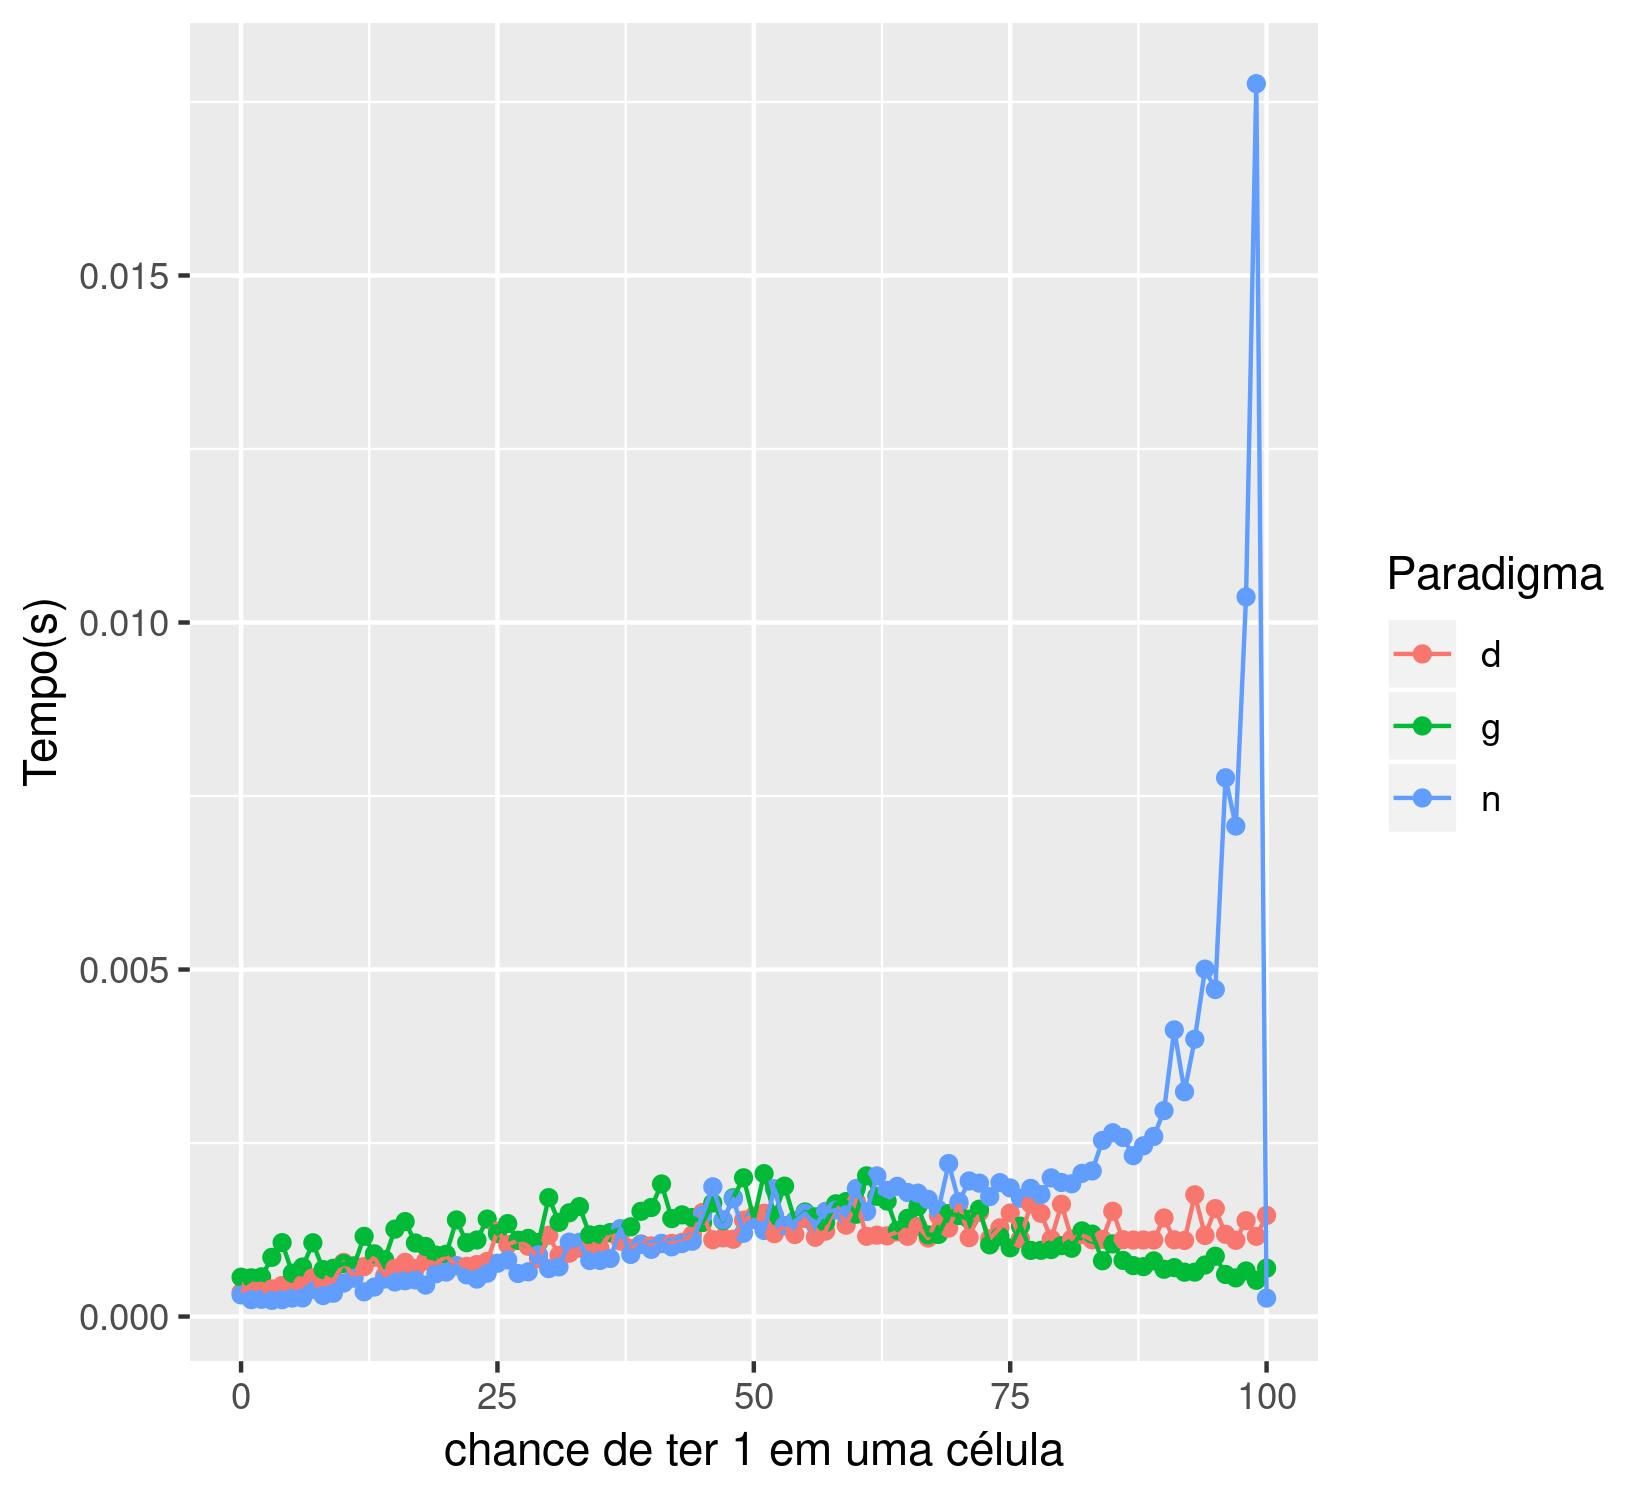
\includegraphics[width=1\textwidth]{tempo-rand-a}
\caption{Todos algoritmos exceto força bruta.}\label{fig:tempo-rand-a}
\end{subfigure}
\begin{subfigure}[b]{.3\textwidth}
\centering
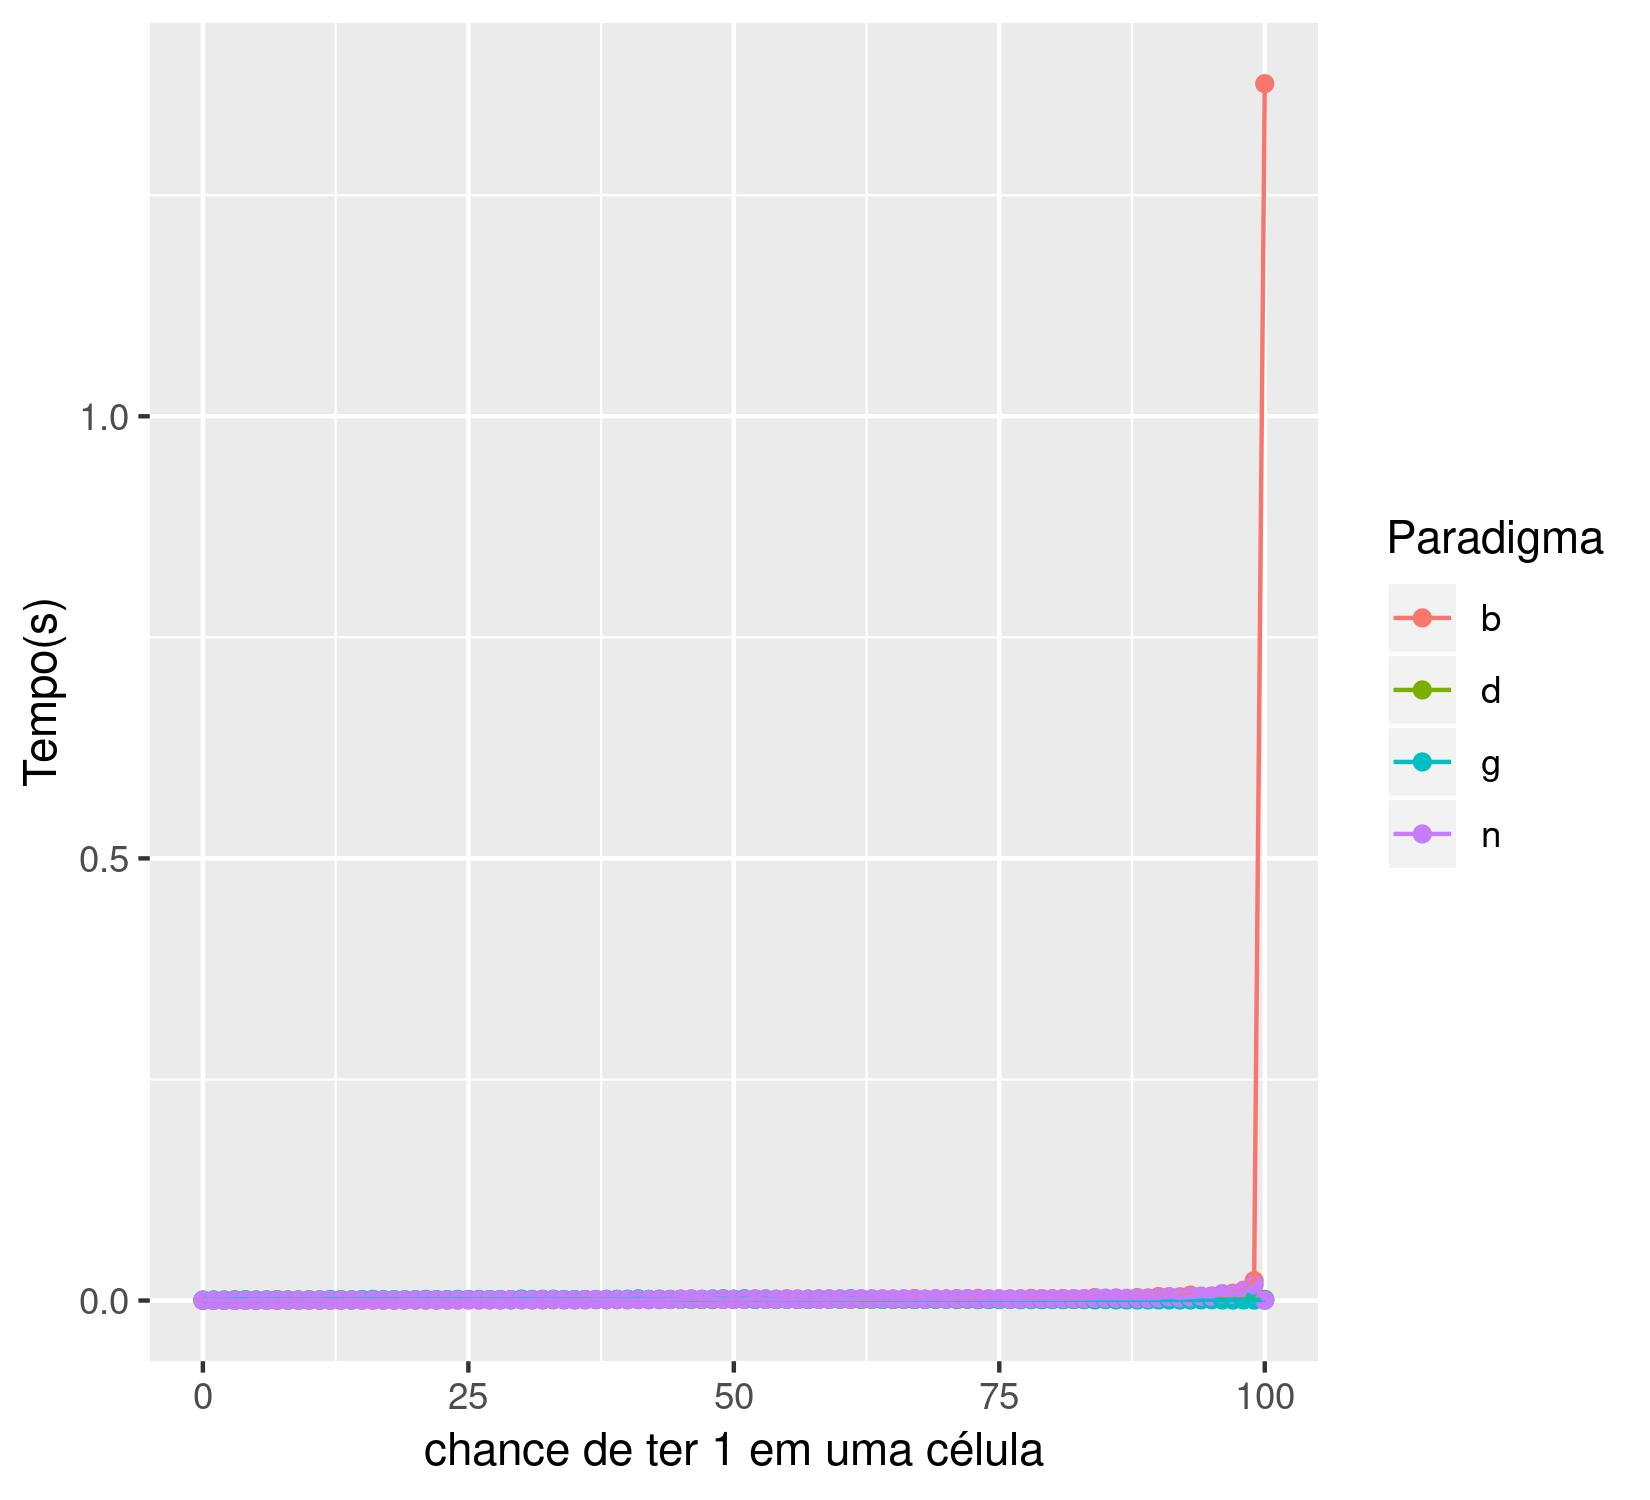
\includegraphics[width=1\textwidth]{tempo-rand-b}
\caption{Todos algoritmos.}\label{fig:tempo-rand-b}
\end{subfigure}
\begin{subfigure}[b]{.3\textwidth}
\centering
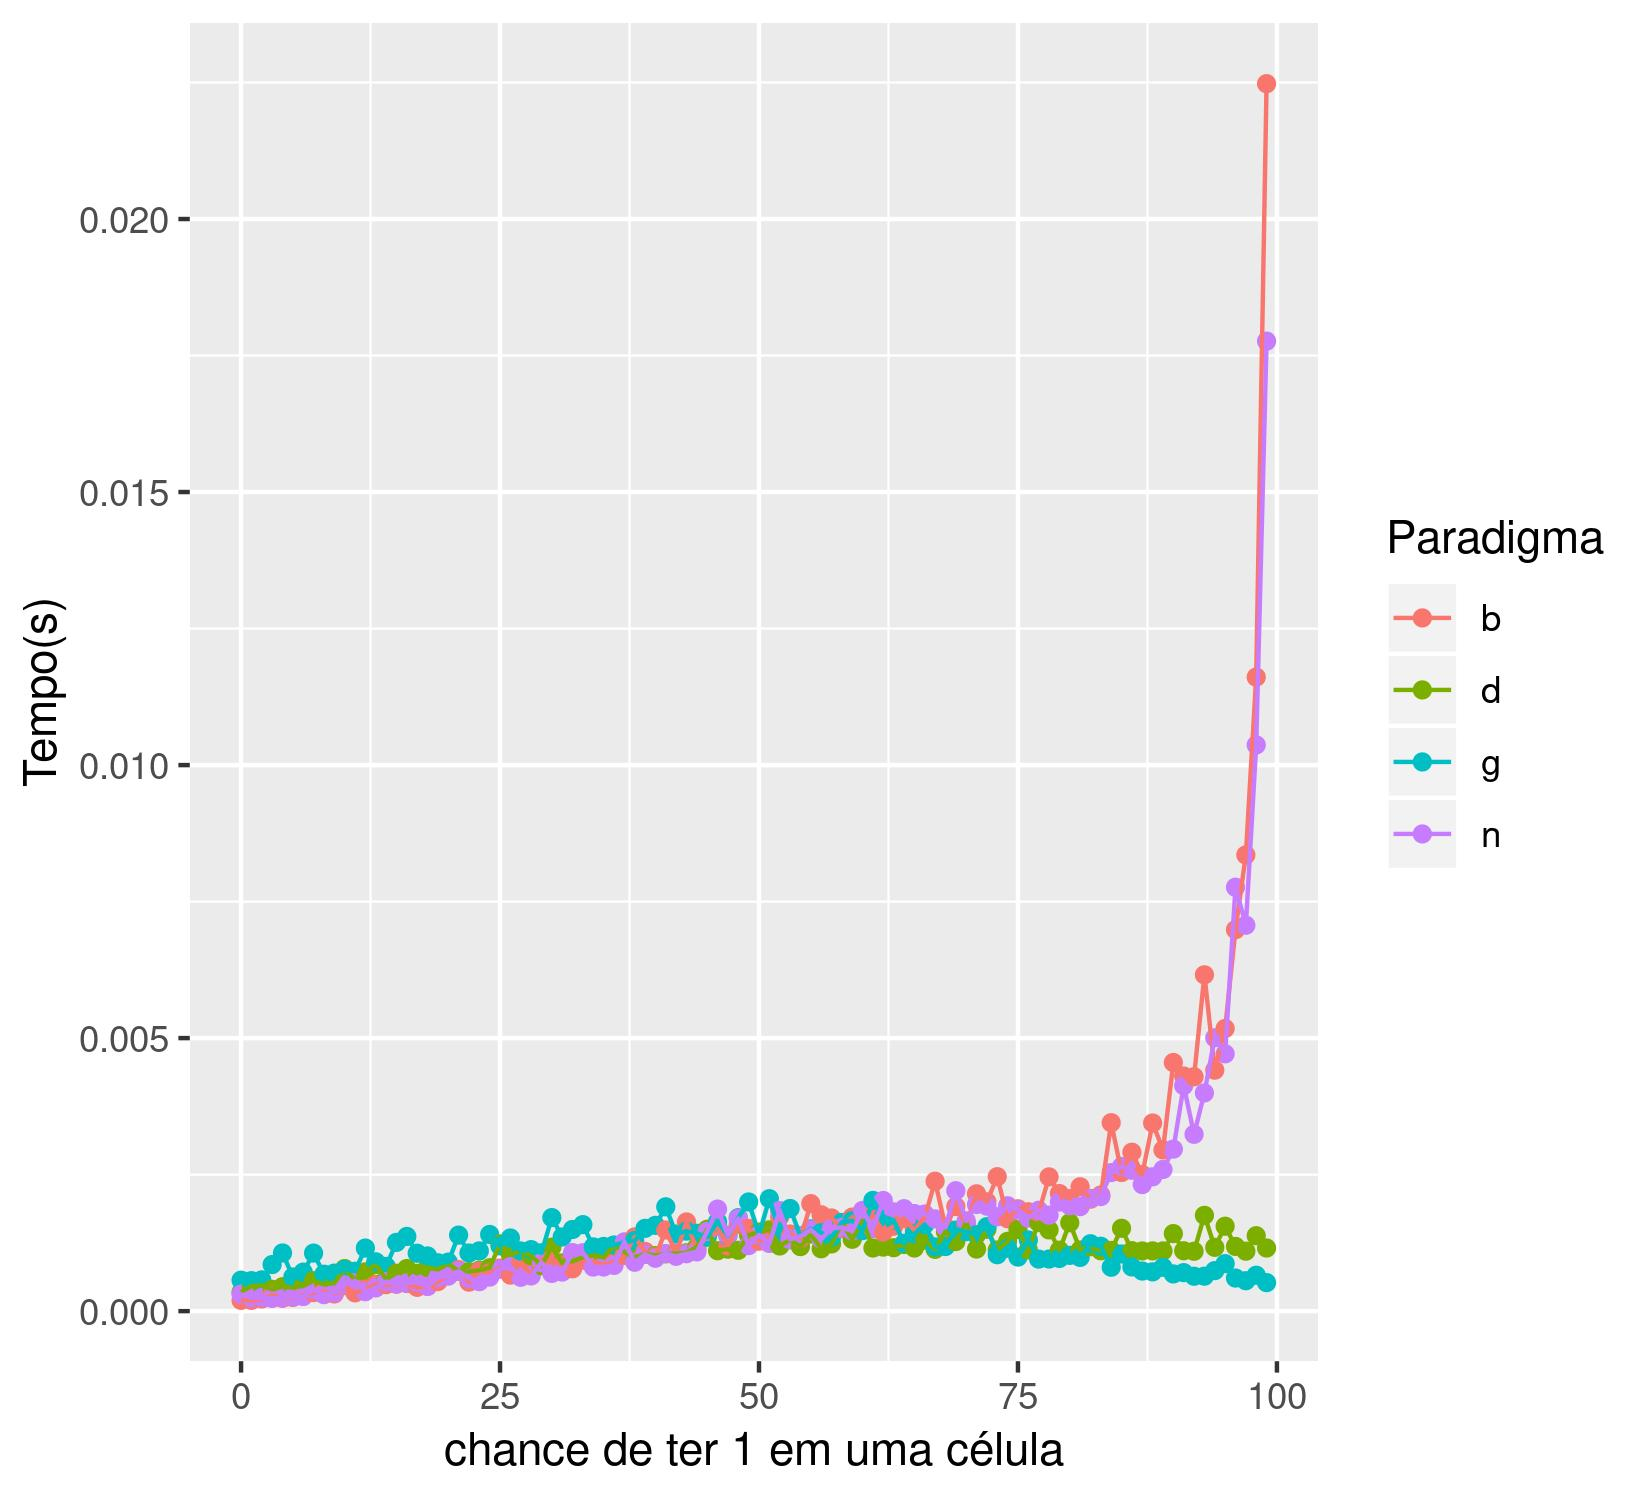
\includegraphics[width=1\textwidth]{tempo-rand-c}
\caption{Todos algoritmos (porcentagem<=99).}\label{fig:tempo-rand-c}
\end{subfigure}

\caption{Tempo por chance de ter um 1 em uma célula.(matriz $200\times 200$)}\label{fig:tempo-rand}
\end{figure}
\end{center}

Primeiramente para checar se as complexidades obtidas que estão na tabela \ref{tab:org6b408f4} são corretas é preciso gerar entradas que exploram o pior caso para obter o pior tempo. Com base no pior tipo de conteúdo em uma entrada de cada algoritmo basta variar a ordem da matriz.

A figura \ref{fig:forcabruta} mostra a regressão polinomial executando o algoritmo força bruta no seu pior caso(matriz completa de 1's). A equação polinomial obtida consegue predizer os valores corretamente, uma equação cubica nesse caso pode obter um resultado bem próximo porém ela falha nos valores iniciais. Pela limitação de obter dados para ordens maiores de matrizes, pois o gráfico já chega mais que 60 segundos por entrada, dificulta mostrar uma falha mais forte em uma possivel regressão cubica. Ou seja na prática o crescimento do tempo é um pouco melhor.

\begin{figure}[htbp]
\centering
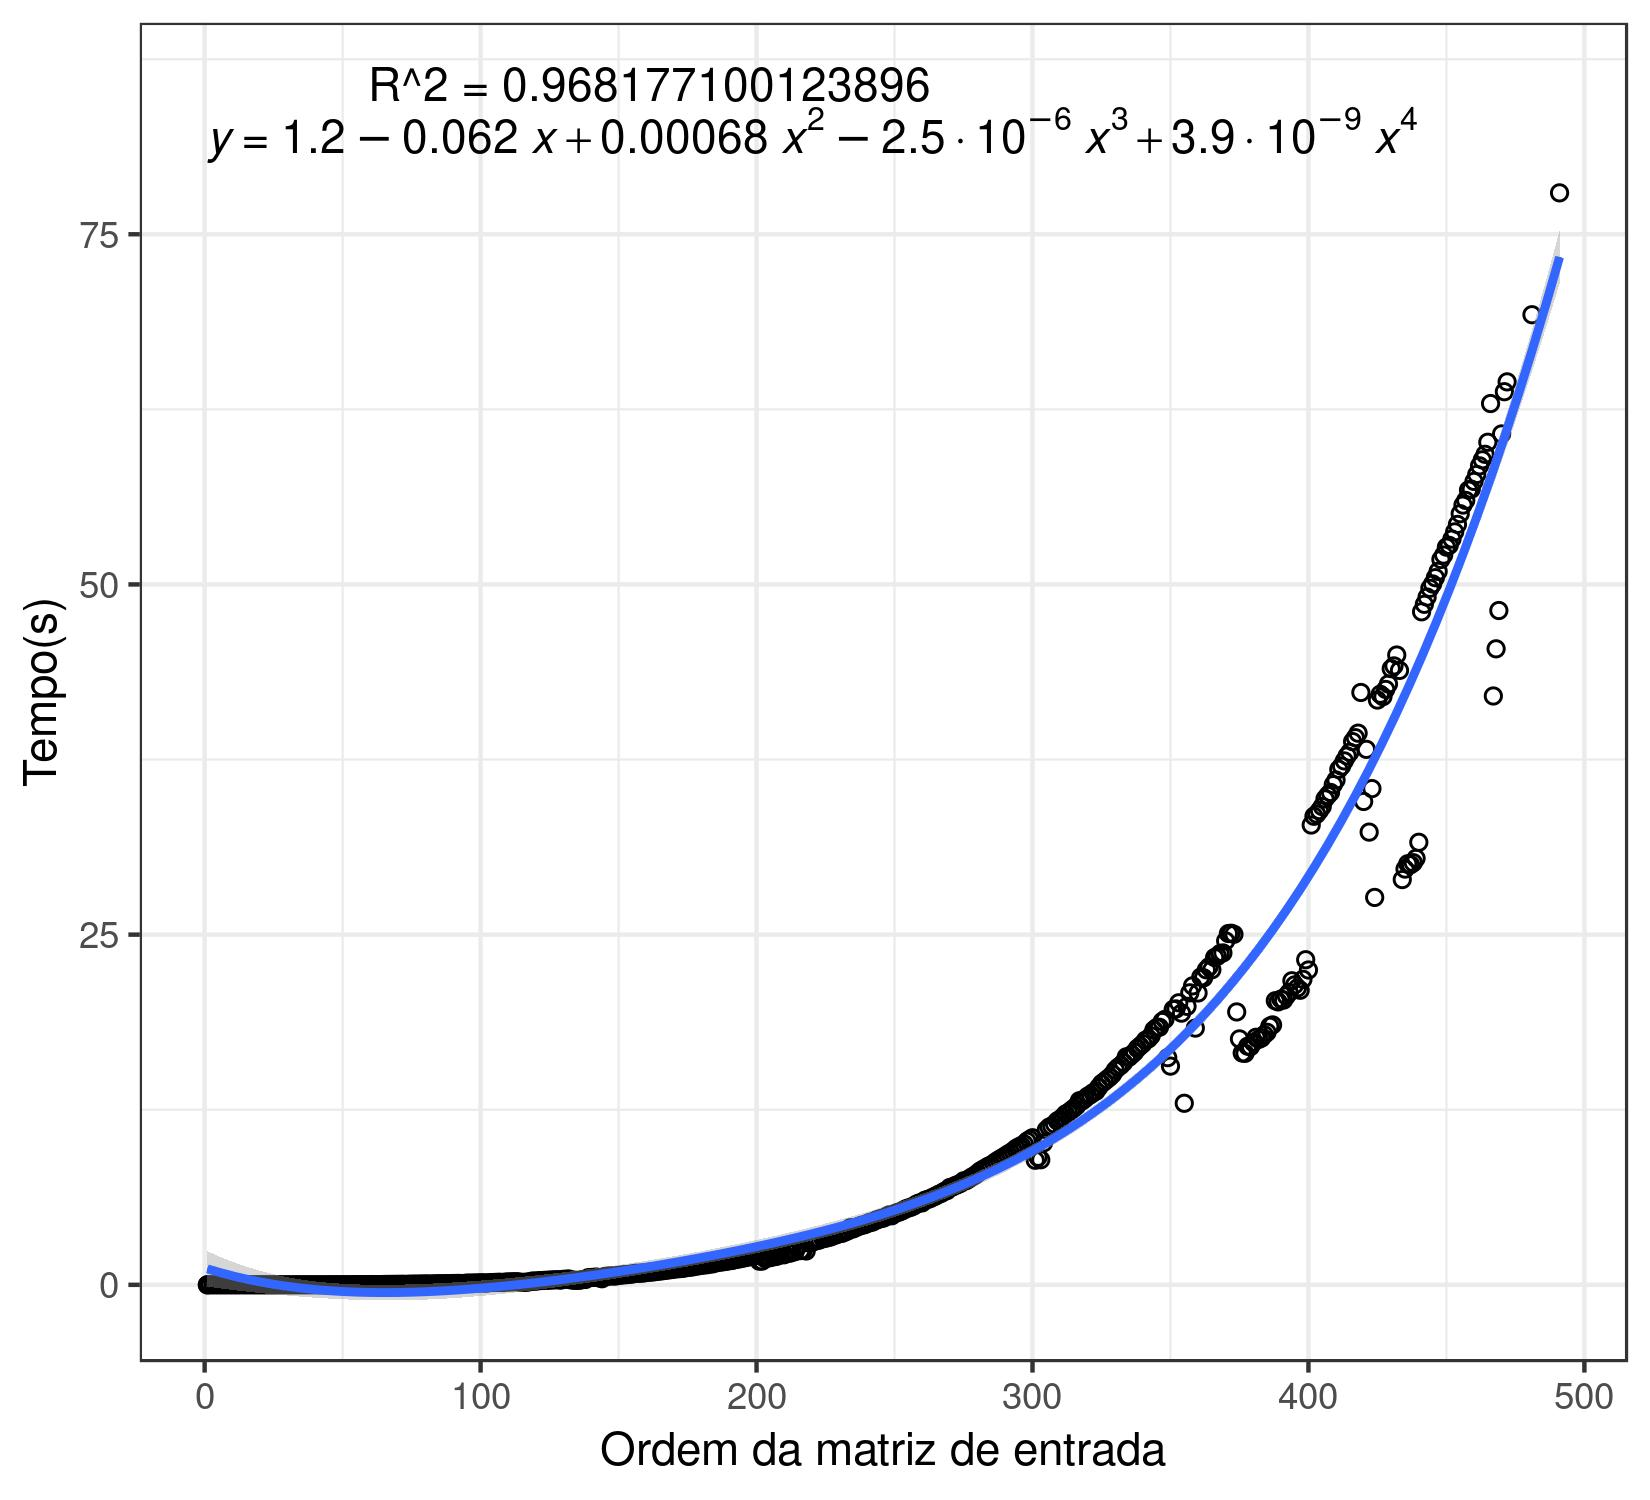
\includegraphics[width=0.33\textwidth]{forcabruta.jpg}
\caption{Tempo força bruta pior caso.\label{fig:forcabruta}}
\end{figure}

A figura \ref{fig:tempo-total} mostra o comportamento do tempo de acordo com o tamanho da entrada para os outros algoritmos, o tempo dos algoritmos tem valores de tempo totalmente discrepantes do algoritmo de força bruta que chega na casa dos minutos.
\begin{center}
\begin{figure}
\begin{subfigure}[b]{.49\linewidth}
\centering
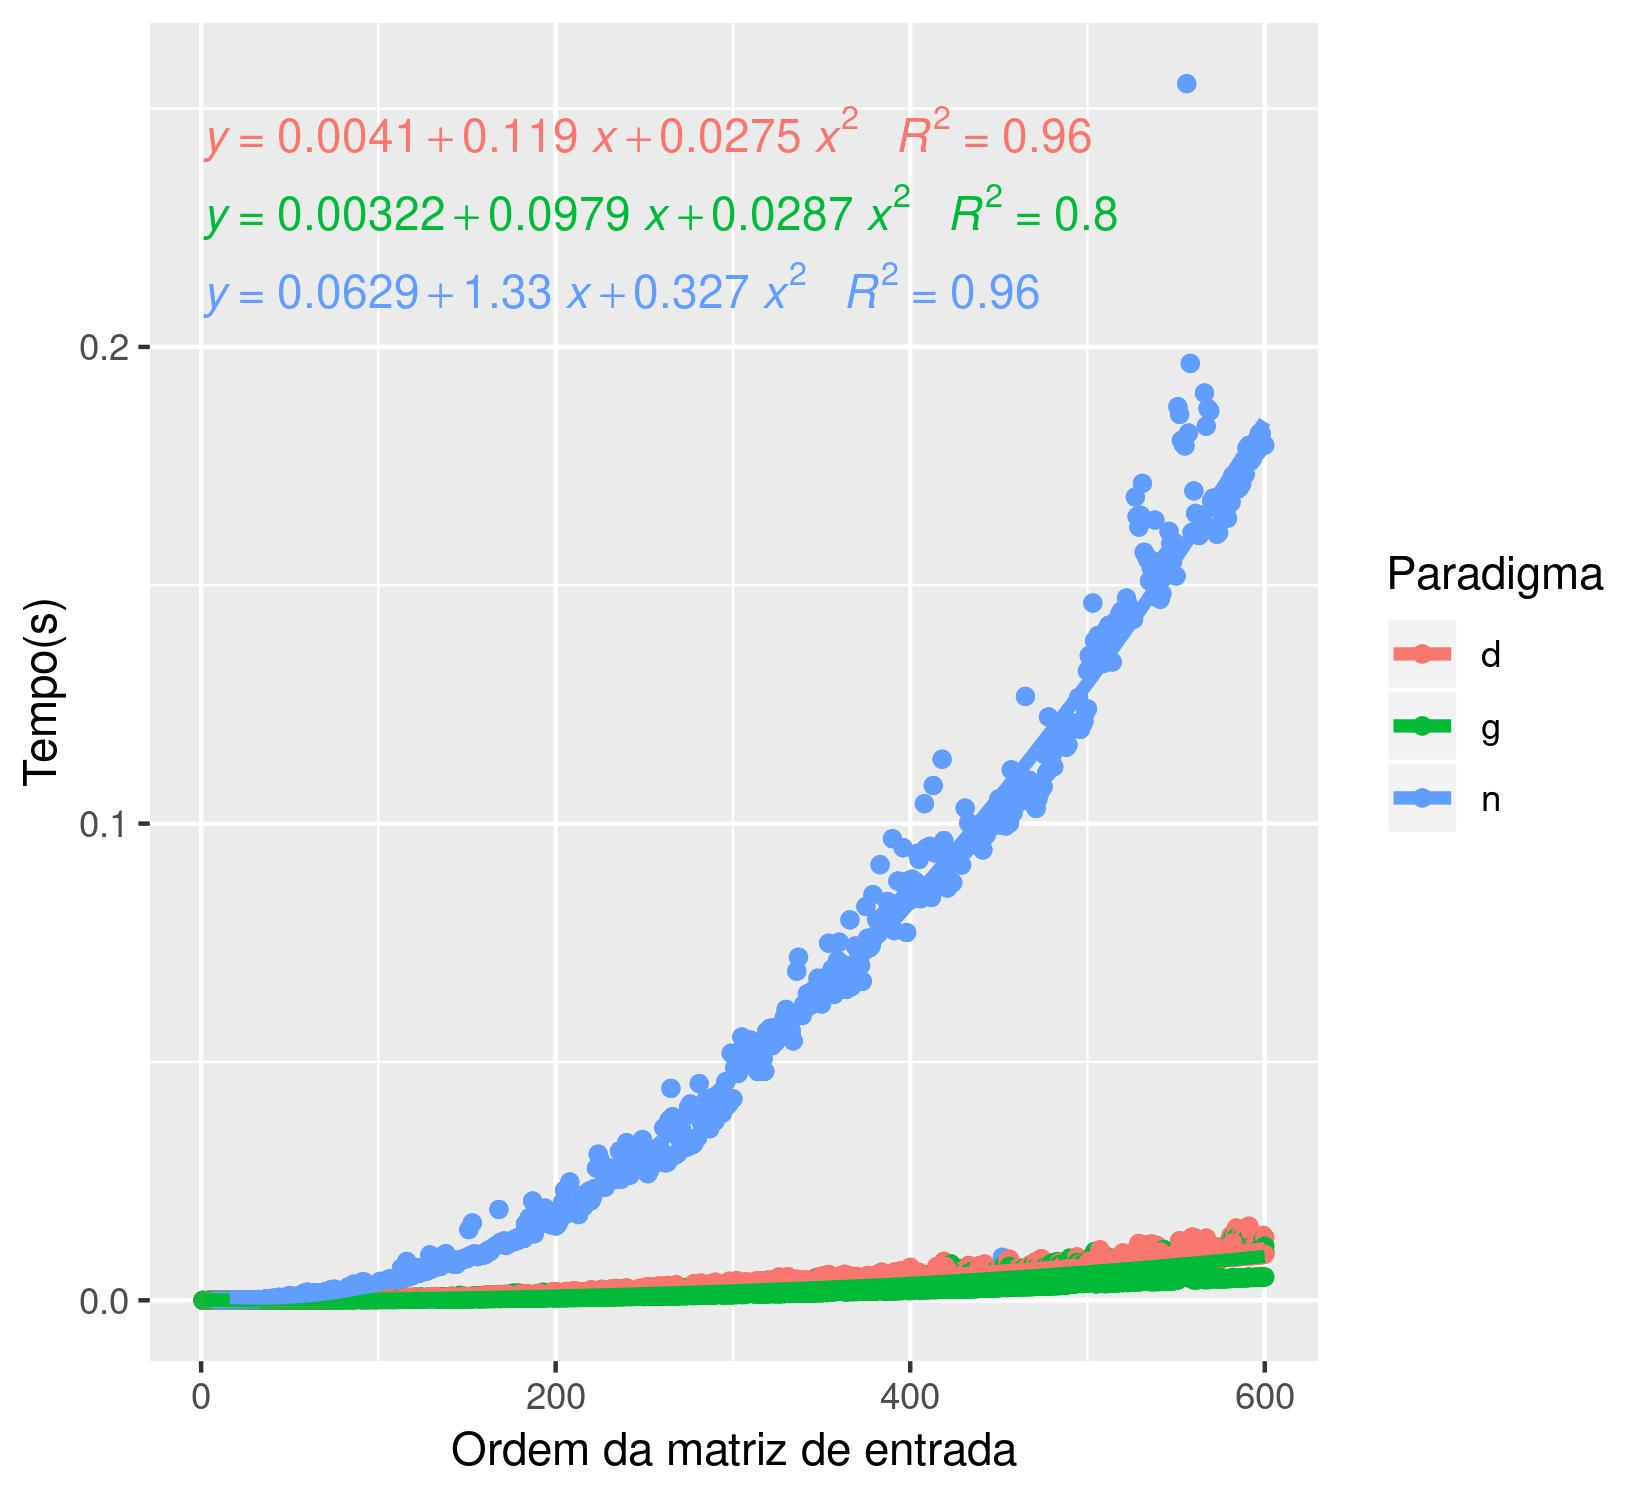
\includegraphics[width=7.5cm]{tempo-total}
\caption{Pior caso.}\label{fig:tempo-total}
\end{subfigure}
\begin{subfigure}[b]{.49\linewidth}
\centering
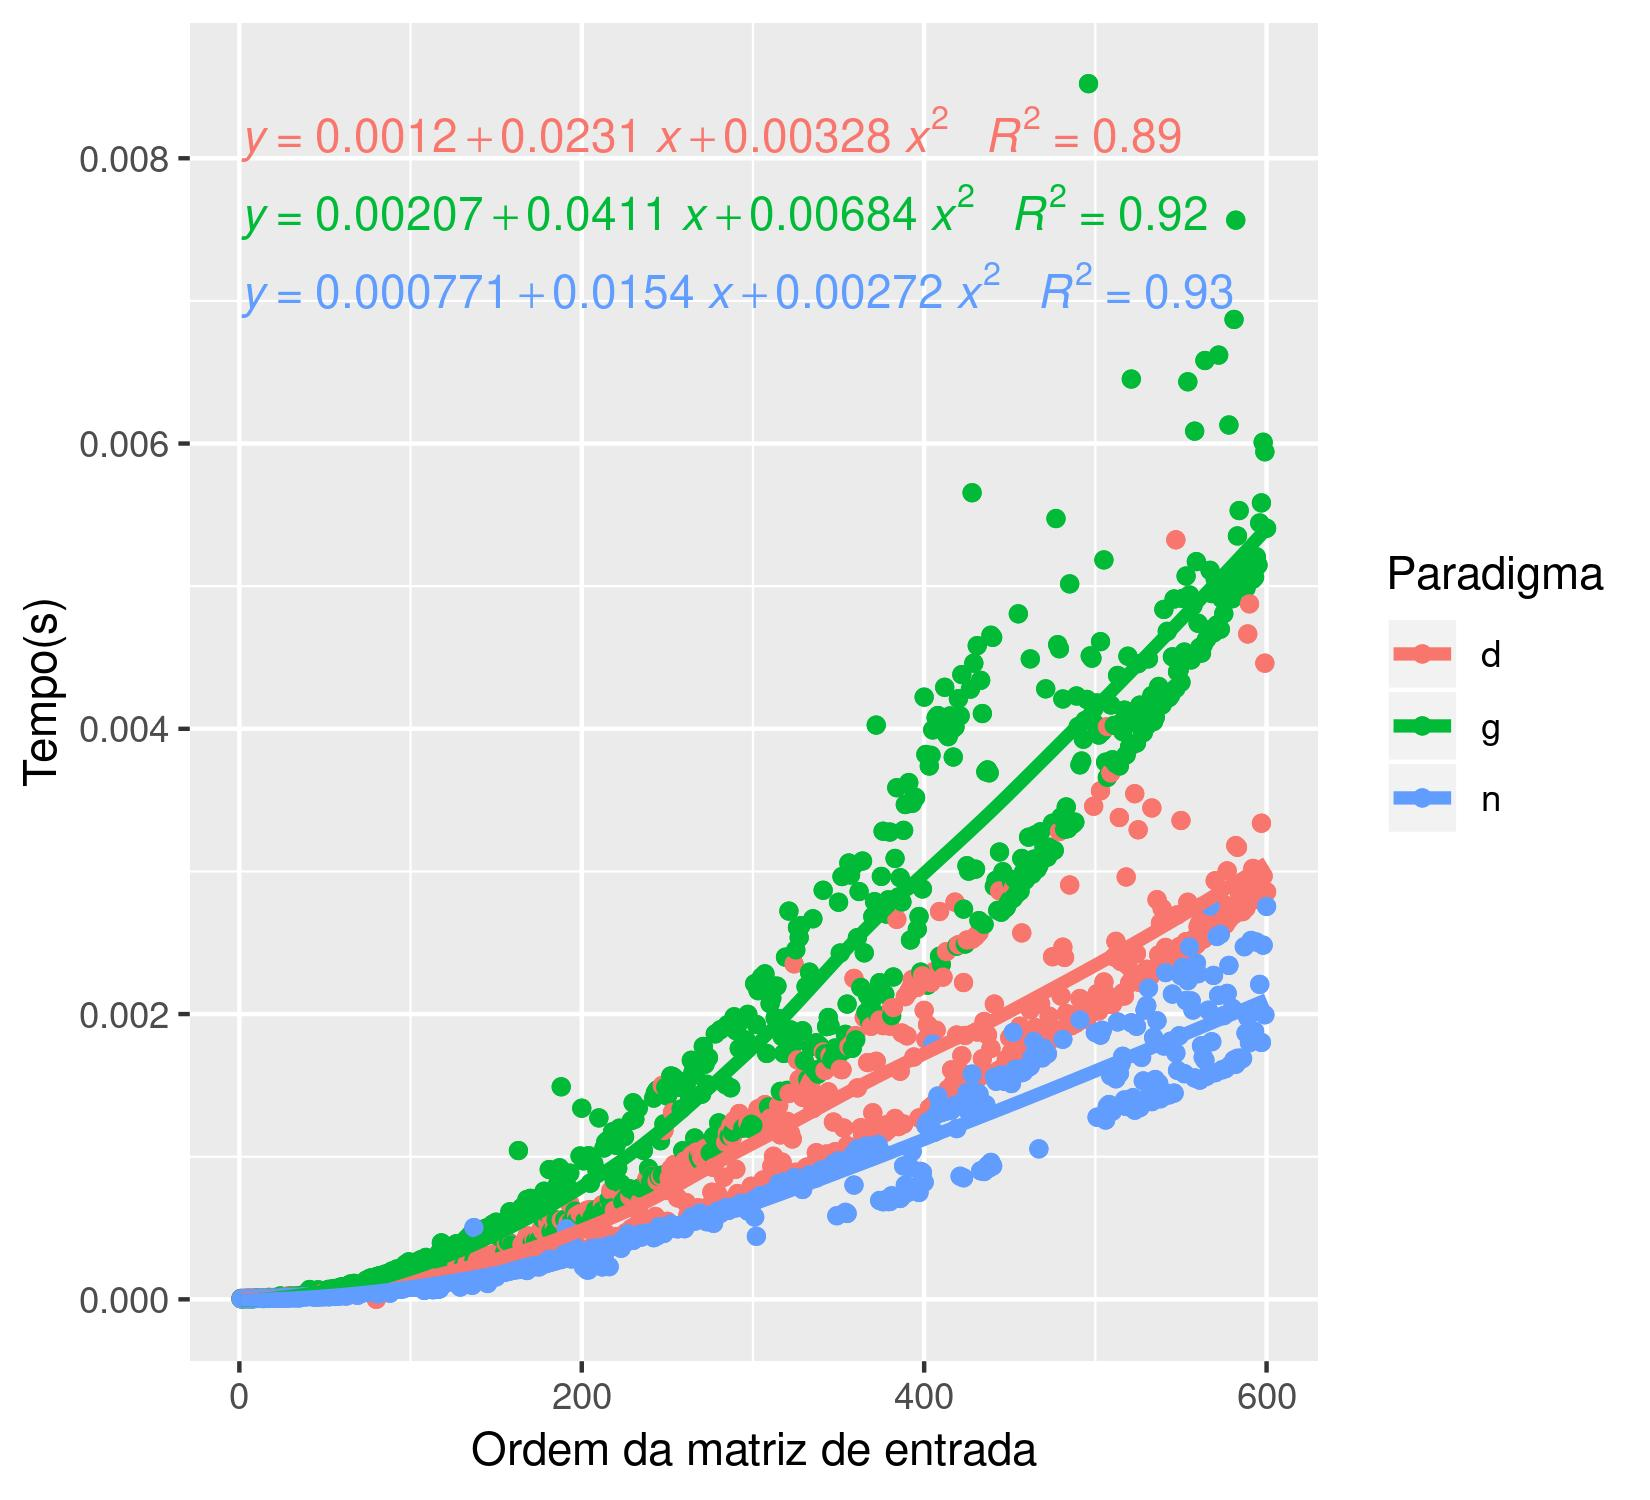
\includegraphics[width=7.5cm]{tempo-best}
\caption{Bons casos.}\label{fig:tempo-best}
\end{subfigure}
\caption{Tempo dos paradigmas rápidos.}
\end{figure}
\end{center}

Devido ao \(R^2\) ter um valor alto nessas regressões de polinômio quadrado pode se concluir que empiricamente foi comprovado a complexidade desses algoritmos. Na prática o \emph{branch and bound} foi muito melhor do que a complexidade obtida na secção de análise de complexidade (\(O(n^4)\)), um polinômio quadrado representou o custo da função com um erro pequeno, ou seja na prática o algoritmo teve uma complexidade perto de \(O(n^2)\).

Também é importante notar que o algoritmo com programação dinâmica se mantém na mesma ordem de tempo independente dos valores de uma matriz porém seus fatores podem ser mudados se a operação mais custosa não for efetuada(\(a_{ij}=0\)). A figura \ref{fig:tempo-best} mostra alguns outros casos de entrada melhores para cada algoritmo e é obtido que o algoritmo de \emph{branch and bound} consegue ter o menor tempo.

Então com o tempo interpretado na prática pode-se ver uma hierarquia de melhores algoritmos em questão de tempo no pior caso, a figura \ref{fig:hierarquiaemp} mostra essa hierarquia.

\begin{figure}
\centering
\begin{tikzpicture}
\node[draw,rectangle,minimum width = 3.5cm] (n1) {Dinâmico};
\node[draw,rectangle,minimum width = 3.5cm,yshift=-0.5cm] (n2) {Guloso};
\node[draw,rectangle,minimum width = 3.5cm,yshift=-1cm] (n3) {Branch and bound};
\node[draw,rectangle,minimum width = 3.5cm,yshift=-1.55cm] (n4) {Força bruta};
\draw[<-,line width=0.3mm,right of = n1,xshift=1cm,yshift=0.27cm] (0,0) -- (0,-2.1) node[anchor=south west] {Rapidez};
\end{tikzpicture}
\caption{Hierarquia de tempo empiríco.}\label{fig:hierarquiaemp}
\end{figure}
\subsection{Espaço}
\label{sec:org98b5d17}
Para provar o tempo do algoritmo principal em relação a memória basta monitorar as alocações feitas pelo algoritmo para cada tamanho de entrada. O monitoramento será feito somente da memória \emph{heap} \cite{osthreeeasypieces} que é a parte da memória onde a alocação dinâmica é feita e o espaço pode-se variar dinamicamente permitindo-se assim obter uma função de complexidade correta.

Pela figura \ref{fig:espaco} o espaço utilizado pelos 3 algoritmos que não o dinâmico utilizam o mesmo espaço e até mesmo tem a mesma regressão polinomial que provém do algoritmo principal na alocação de memória para a matriz de entrada. Já o algoritmo dinâmico tem a complexidade \(O(n^2)\) do algoritmo principal mais \(O(n^2)\) na matriz auxiliar logo seu custo de espaço é maior porém continua tendo complexidade assintótica \(O(n^2)\) assim como todos outros paradigmas considerando o programa principal.

Então é necessário ser cauteloso com a utilização do algoritmo dinâmico para grandes matrizes pois pode ser visto que o custo de espaço tem fatores em sua função que o fazem crescer de forma muito maior que os outros algoritmos. 

\begin{figure}[htbp]
\centering
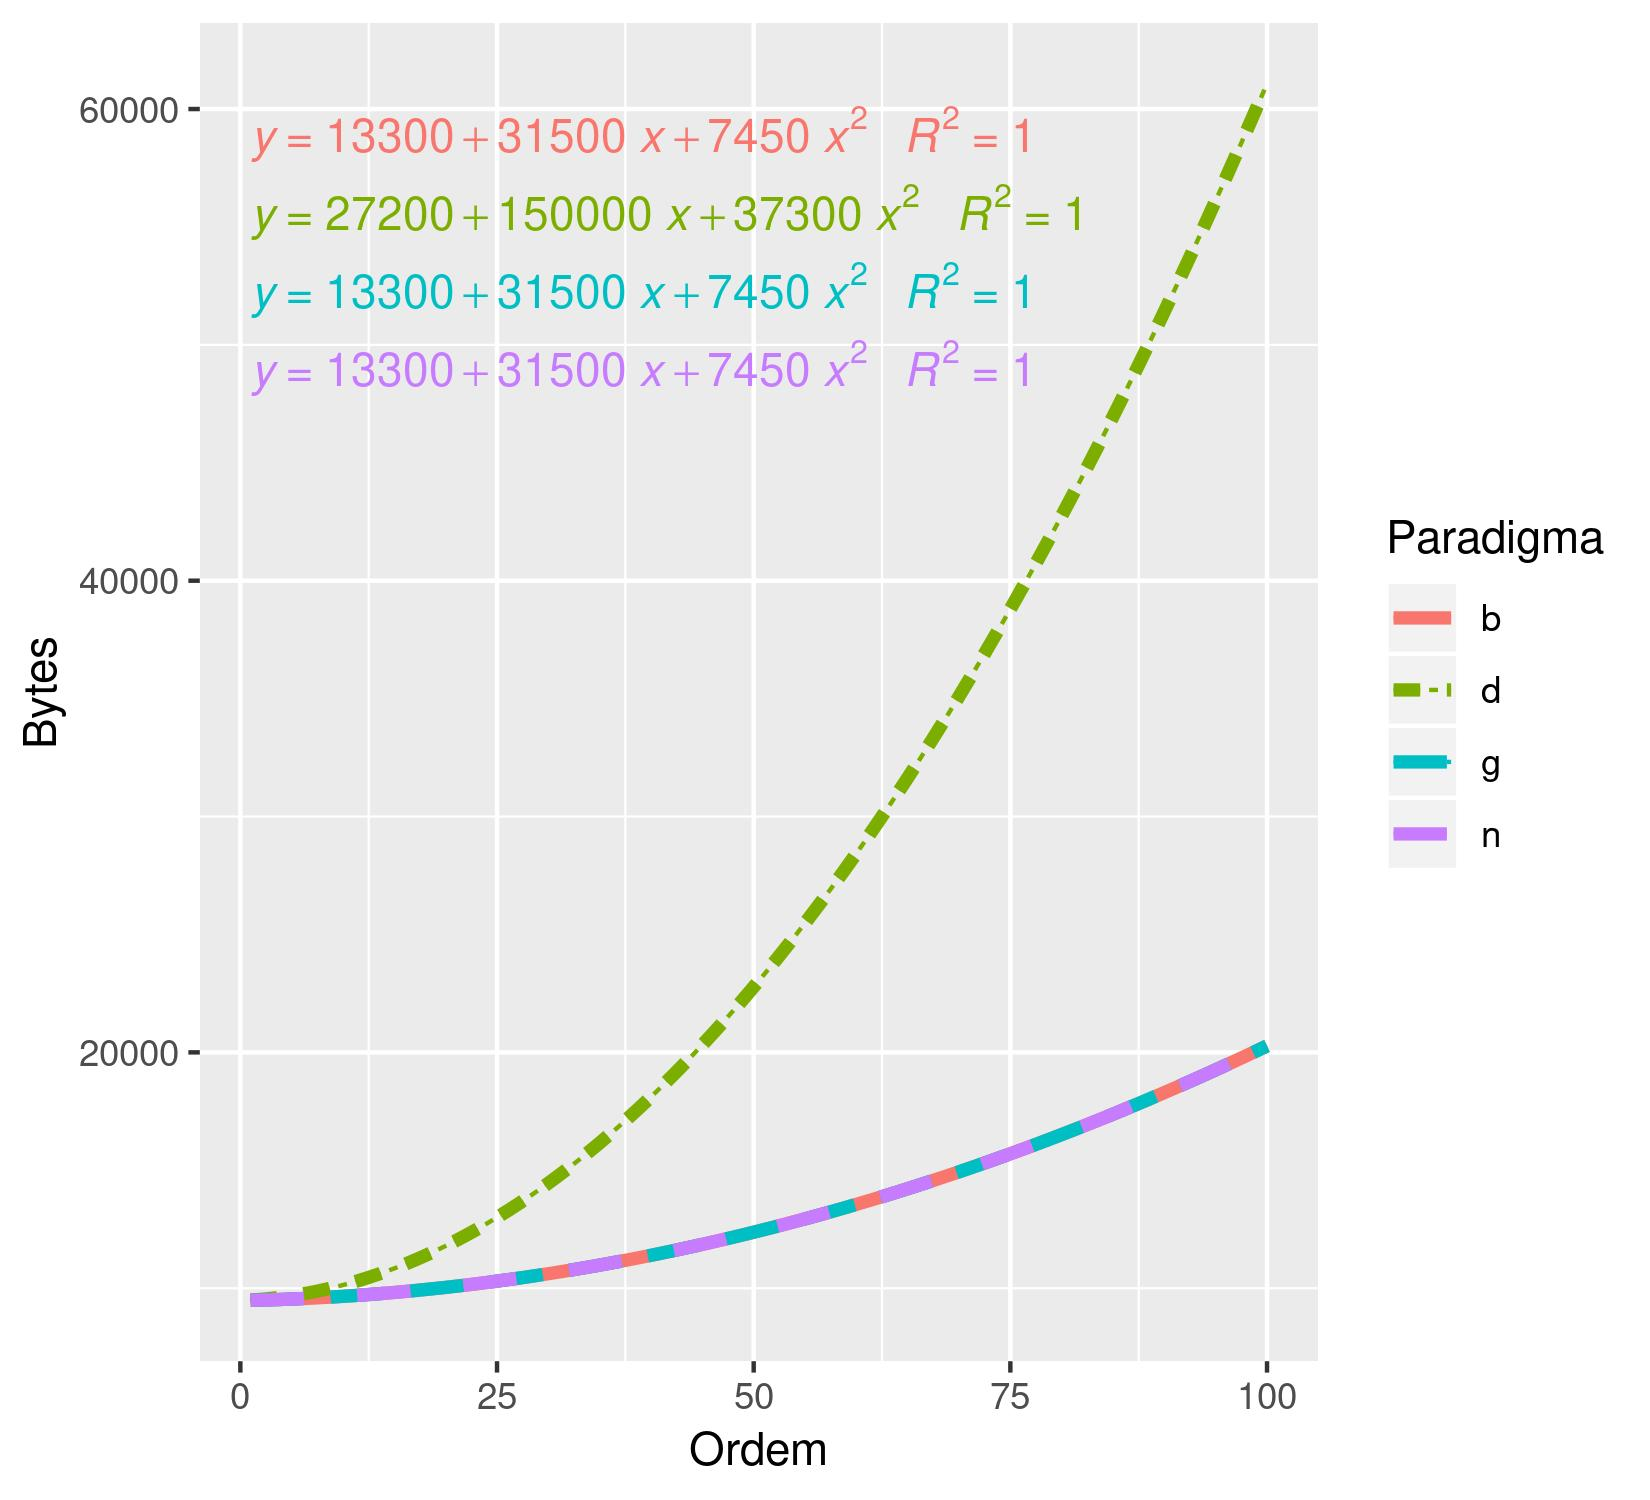
\includegraphics[width=0.33\textwidth]{espaco.jpg}
\caption{Espaço usado pelos paradigmas.\label{fig:espaco}}
\end{figure}

Pelas funções de complexidade obtidas com um \(R^2=1\) é possível predizer o quanto de espaço o algoritmo irá utilizar para cada ordem de entrada o que pode ser uma coisa útil para aplicação do algoritmo na prática. Um exemplo de aplicação dessa função prediria se o algoritmo gasta mais memória do que o computador atual possui disponível então se sim usa outro algoritmo que seja possível, esse processo é ilustrado na figura \ref{fig:spacepredict}. É importante lembrar que a função de complexidade obtida varia de arquitetura para arquitetura e é um cuidado que deve ser tomado pois os tipos de dados primitivos podem ter tamanhos diferentes.
\begin{figure}
\centering
\begin{tikzpicture}[node distance = \myDistance, auto]
\node [draw,ellipse] (ini) {Ordem};
\node [block,right of = ini] (poly) {Função custo espaço dinâmico};
\node [draw,ellipse,right of = poly] (bytes) {Bytes};
\node [decision,right of = bytes] (check) {Bytes>Memória};
\node [block,above right of = check] (yes) {Algoritmo secundário(Mesmo processo)};
\node [block,below right of = check] (no) {Dinâmico};

\path [line] (ini) -- (poly);
\path [line] (poly) -- (bytes);
\path [line] (bytes) -- (check);
\path [line] (check) -- (yes) node [midway, yshift= -0.1cm ,above] (TextNode) {Verdadeiro};
\path [line] (check) -- (no) node [midway, yshift= -0.1cm ,above] (TextNode) {Falso};
\end{tikzpicture}
\caption{Utilização da função de custo de espaço.}\label{fig:spacepredict}
\end{figure}

\subsection{Estratégia gulosa}
\label{sec:orgc0f73a7}
A taxa de acerto do algoritmo guloso como é mostrado na figura \ref{fig:greedy-ac} é muito baixa, ele somente obtém uma solução ótima quando o tamanho da matriz é muito baixo. Porém é importante se atentar ao fato de que os dados de entrada foram com matrizes preenchidas de forma aleatória e o problema a ser resolvido vem da realidade que tem padrões e não possui toda essa estrutura aleatória que faz com que a estrategia seja muito ineficiente.

Com entradas com mais ordem e algo mais parecido com placentas na realidade o algoritmo possui soluções melhores, isso pode ser visto comparando os diagramas de caixa na figura \ref{fig:barplox-greedy}.

\begin{figure}[htbp]
\centering
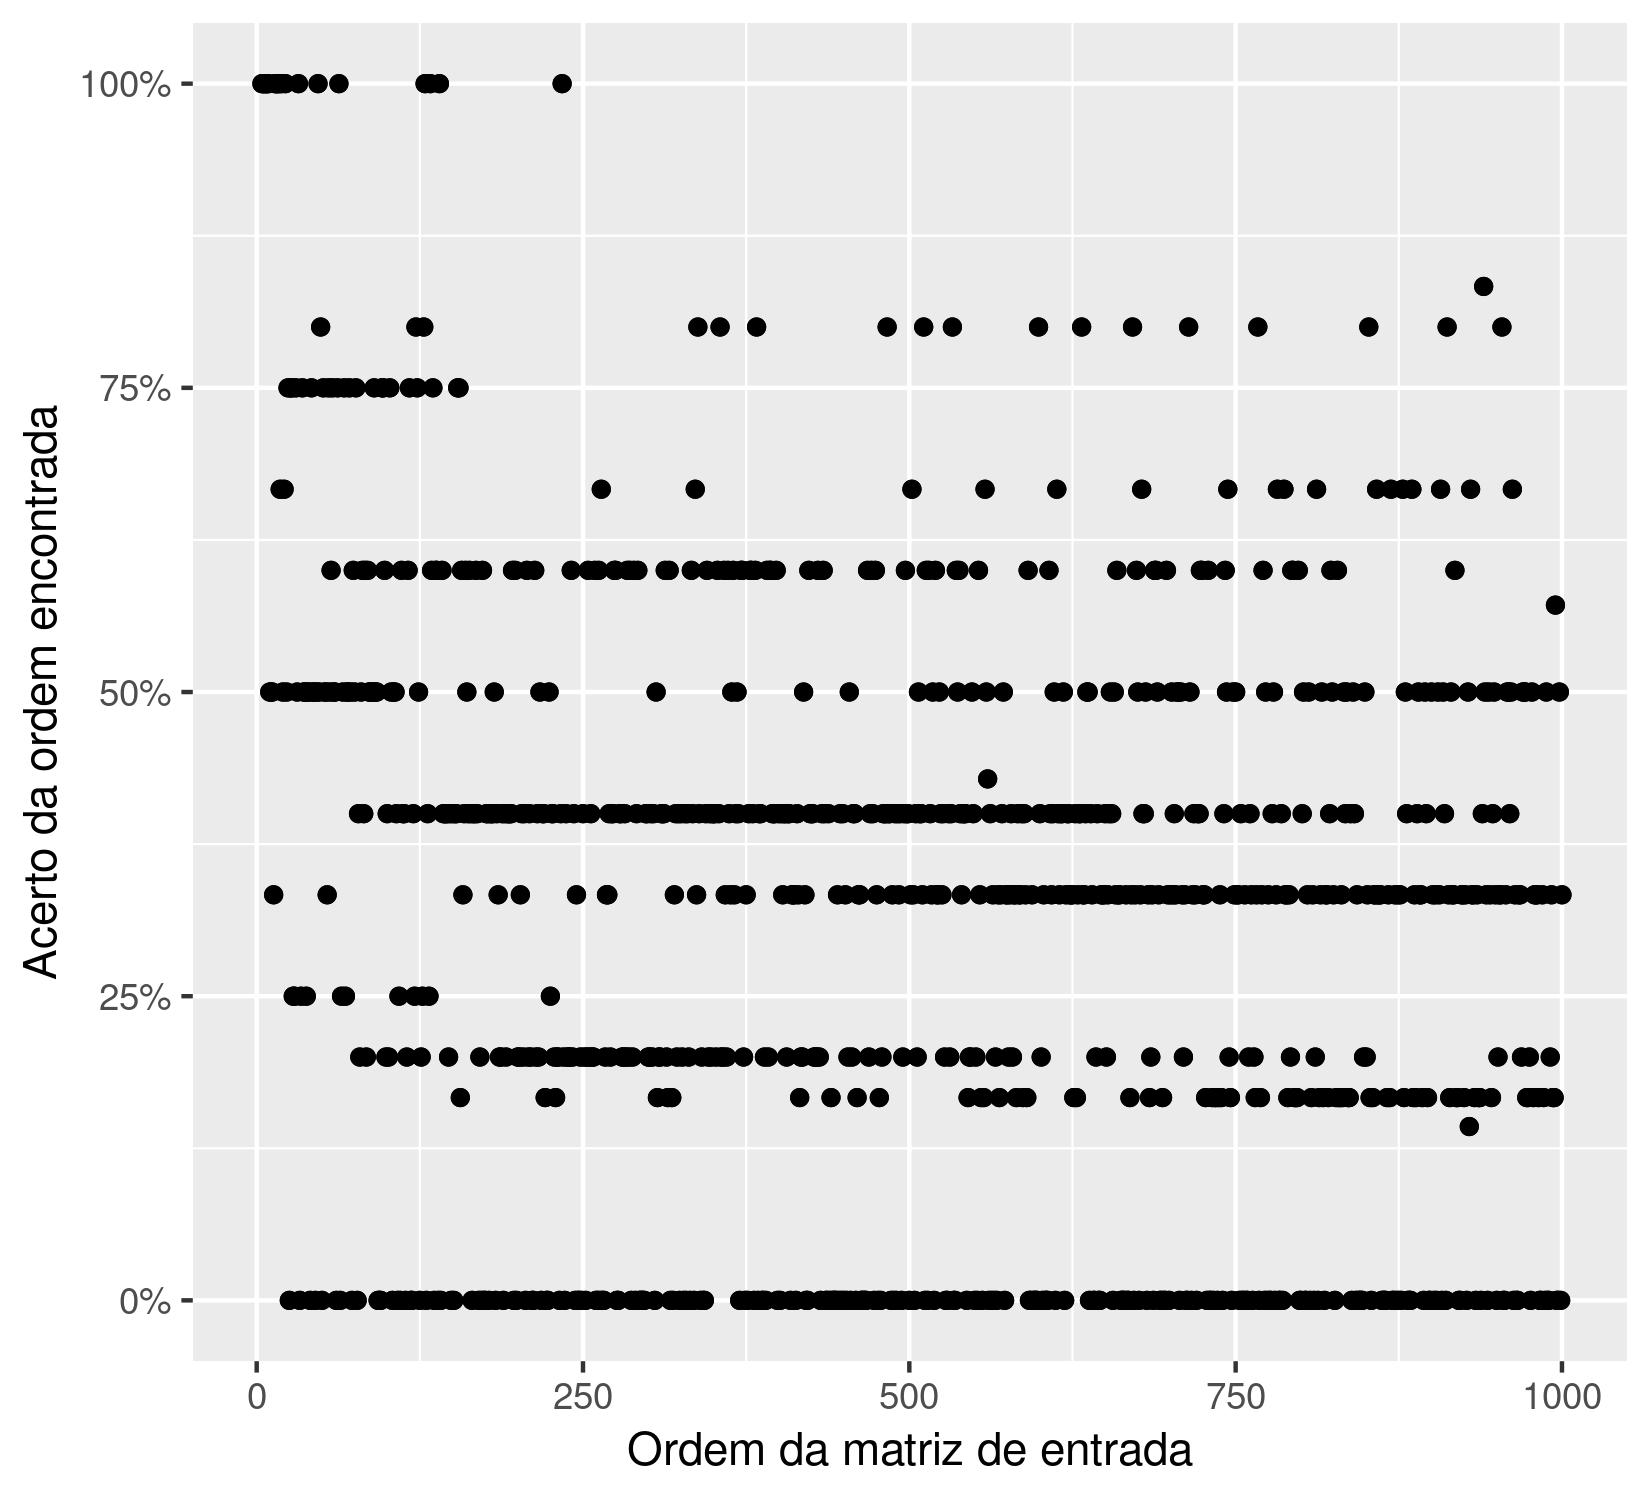
\includegraphics[width=0.28\textwidth]{greedy-ac.jpg}
\caption{Taxa de acerto com estratégia gulosa.\label{fig:greedy-ac}}
\end{figure}

\begin{center}
\begin{figure}
\begin{subfigure}[b]{.49\linewidth}
\centering
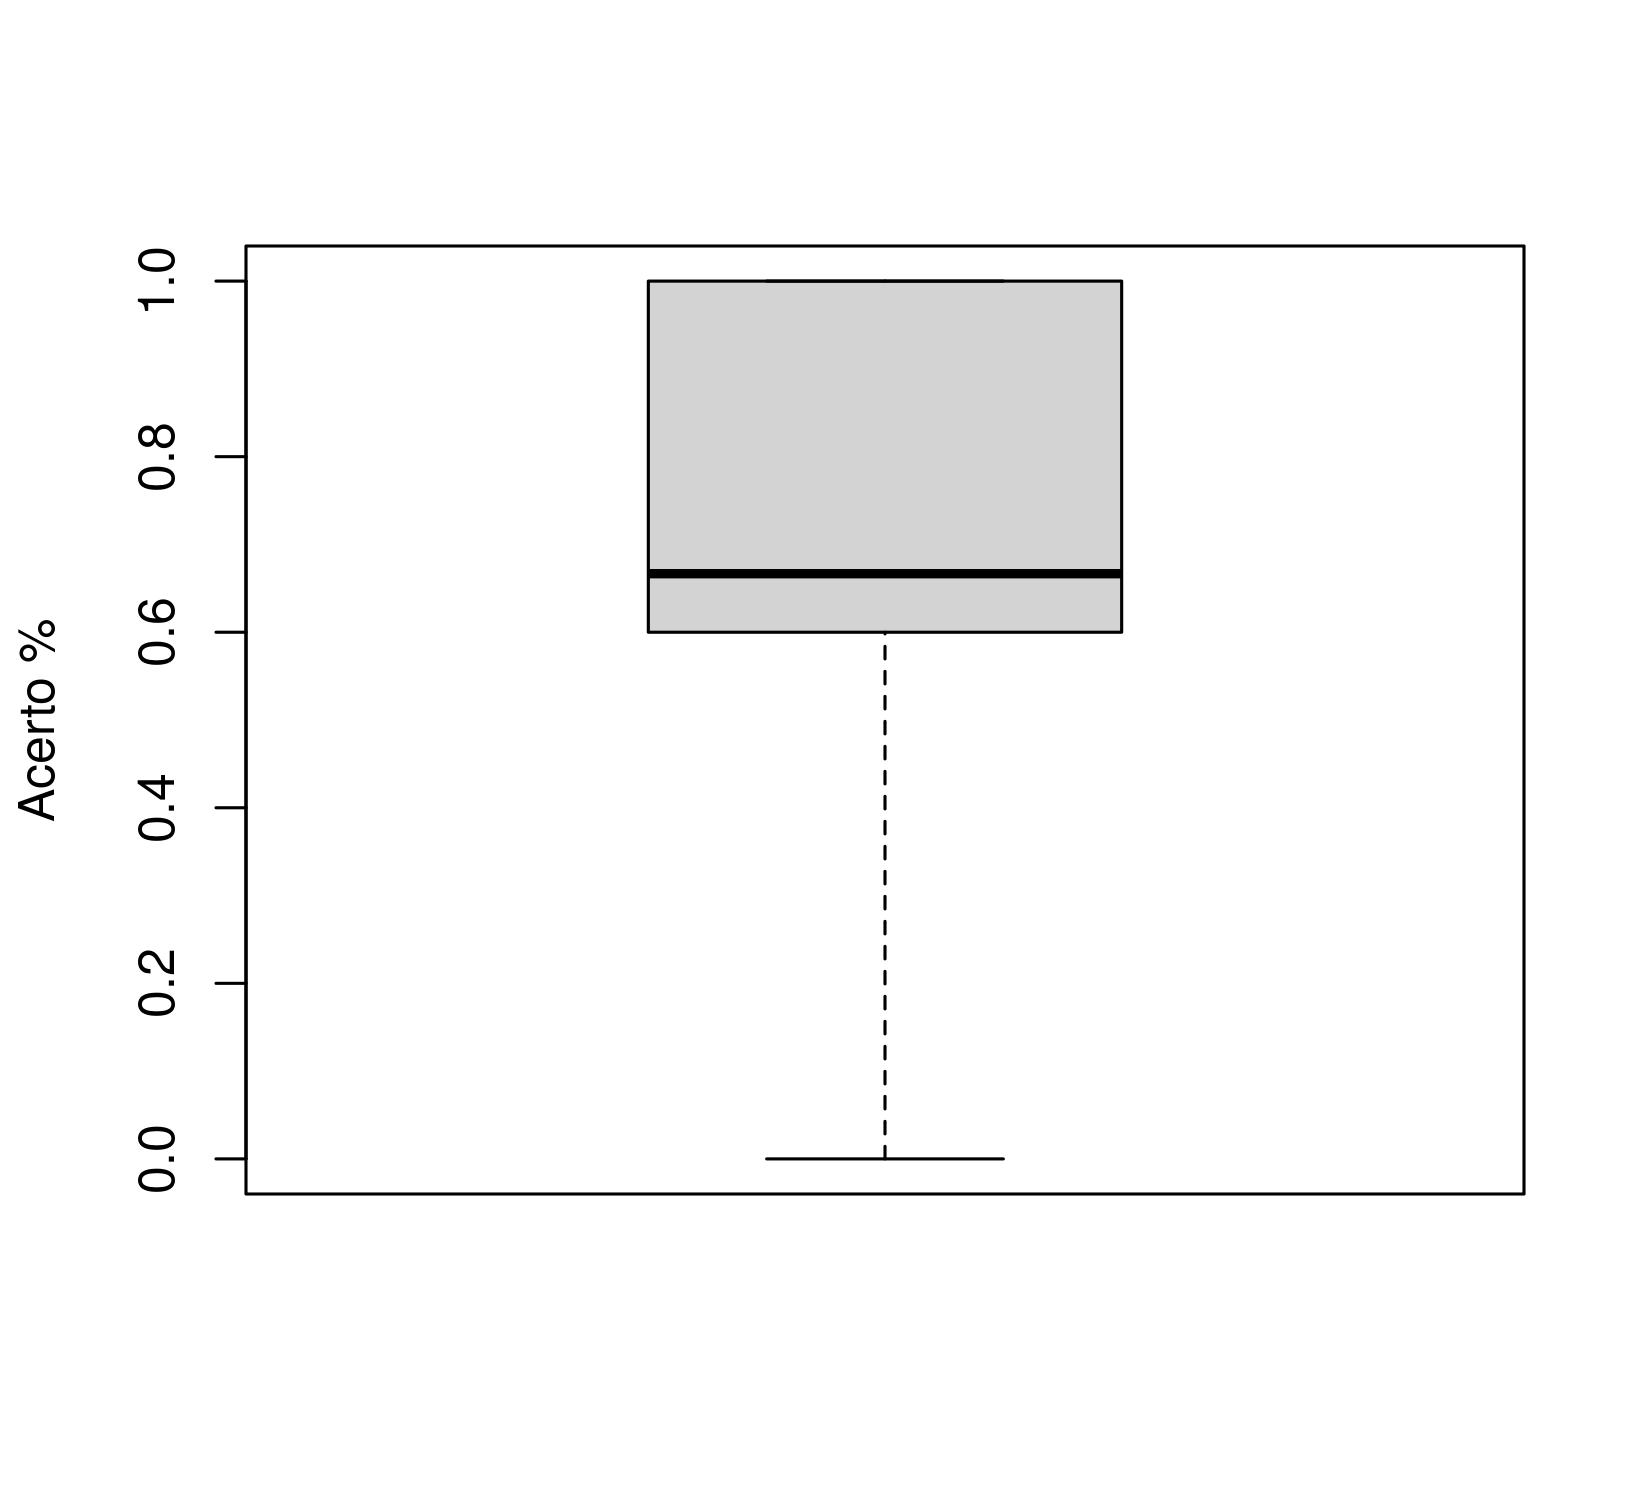
\includegraphics[width=\linewidth/2]{bar-greedy-ac-best}
\caption{Entradas realistas.(10 amostras)}\label{fig:bar-greedy-ac-best}
\end{subfigure}
\begin{subfigure}[b]{.49\linewidth}
\centering
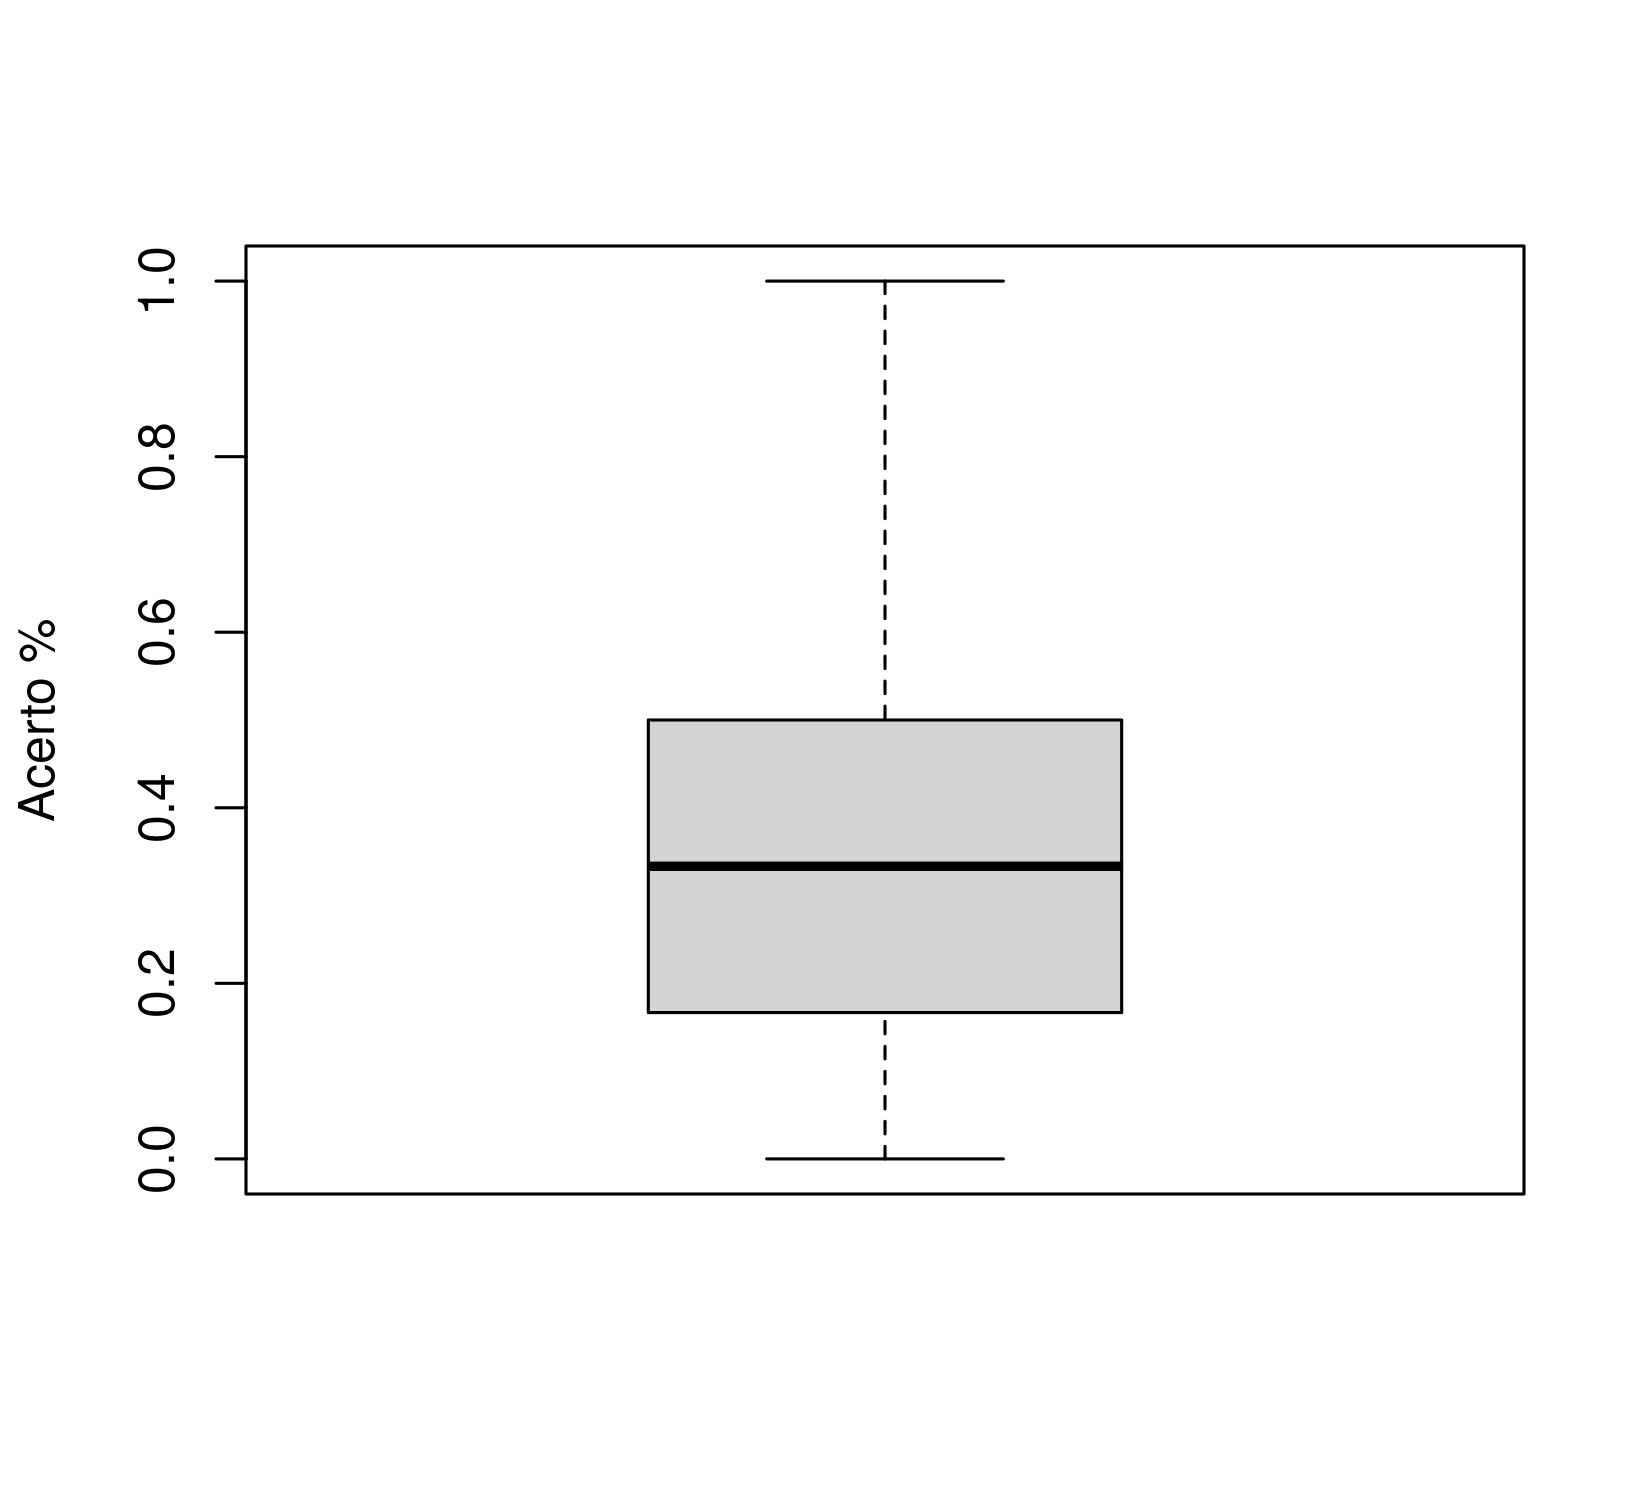
\includegraphics[width=\linewidth/2]{bar-greedy-ac}
\caption{Entradas aleatórias.}\label{fig:bar-greedy-ac}
\end{subfigure}
\caption{Taxa de acerto da estratégia gulosa.}\label{fig:barplox-greedy}
\end{figure}
\end{center}

\section{Conclusão}
\label{sec:orga273154}

Com o trabalho foi possível observar que o problema possui um algoritmo que resolve-o com complexidade de tempo de \(O(n^2)\) e com custo de espaço \(O(n^2)\), diferentemente do força bruta com tentativa e erro que tem complexidade assintótica de tempo de \(O(n^4)\) e se mostrou ineficiente, garantindo solução ótima por meio de programação dinâmica e se mostrando o algoritmo mais estável por meio dos resultados observados, porém por ser estável em alguns casos o algoritmo que utiliza \emph{branch and bound} apresenta tempos melhores porém como o pior caso deve ser sempre o considerado é melhor utilizar o algoritmo com programação dinâmica. A estratégia gulosa não garante uma solução ótima e nos testes o seu erro foi bem grande, logo não é nem um pouco ideal ser utilizada, somente caso seja uma matriz extremamente grande e não seja possível aplicar o \emph{branch and bound} ou o dinâmico.

É bem difícil que para a aplicação proposta uma matriz de entrada esteja quase toda completa com 1's, logo o \emph{branch and bound} pode se sair melhor ainda com uma certa garantia devido a esse possivel padrão de problema de entrada. Se em um trabalho futuro for verificado que a placenta tenha em média 75\% para menos de material sólido o algoritmo \emph{branch and bound} se torna uma alternativa mais viável para ser utilizado ao invés do guloso, isso dito com base nos gráficos mostrados.

Também foi possível obter uma função de complexidade de espaço para os algoritmos empiricamente e com isso foi proposto uma utilização para esse dado que é a predição de estouro da memória para o algoritmo dinâmico e forçar a utilização de algum dos outros algoritmos caracterizado como o melhor. Por meio dos resultados empíricos o \emph{branch and bound} se mostrou o segundo algoritmo mais viável para utilização caso não seja possível a utilização do dinâmico, garante uma solução ótima e também tem um tempo bem similar ao guloso, em alguns casos sendo mais rápido. O guloso nos testes teve um erro grande para entradas aleatórias porém com entradas com uma forma mais similar a uma placenta o algoritmo da soluções melhores.



\bibliographystyle{plain}
\bibliography{doc}
\end{document}
